%%%%%%%%%%%%%%%%%%%%%%%%%%%%%%%%%%%%%%%%%%%%%%%%%%%%%%%%%%%%%%%%%%%%%%
% Quantum-Safe Cryptography Report: Building & Installing New Signature Algorithm
%%%%%%%%%%%%%%%%%%%%%%%%%%%%%%%%%%%%%%%%%%%%%%%%%%%%%%%%%%%%%%%%%%%%%%

\documentclass[11pt,a4paper]{report}

%-------------------------
% Package Imports
%-------------------------
\usepackage[margin=1in]{geometry}            % Page margins
\usepackage{graphicx}                        % Images and logos
\usepackage{titlesec}                        % Custom section formatting
\usepackage{fancyhdr}                        % Headers and footers
\usepackage{setspace}                        % Line spacing
\usepackage{hyperref}                        % Hyperlinks
\bibliographystyle{alpha}
\usepackage{enumitem}                        % Customized lists
\usepackage{lmodern}                         % Enhanced fonts
\usepackage{xcolor}                          % Color definitions
\usepackage{array}                           % Table formatting
\usepackage{listings}                        % For code listings

\usepackage{multicol}

\usepackage{dirtree}
% adjust the indent size if you like:
%\renewcommand{\DTbaselinestretch}{1.1}
%\setcounter{DTlinenosize}{0}6

\usepackage{tikz}
\usetikzlibrary{arrows.meta,calc,positioning}
\usetikzlibrary{arrows}			%% Include regular arrows
% alternative * arrow
\pgfarrowsdeclare{* new}{* new}
{
  \ifdim\pgfgetarrowoptions{* new}<0pt%
    \pgfutil@tempdima=0.4pt%
    \advance\pgfutil@tempdima by.2\pgflinewidth%
    \pgfutil@tempdimb=5.5\pgfutil@tempdima%
    \advance\pgfutil@tempdimb by\pgflinewidth%
    \pgfarrowsleftextend{+-\pgfutil@tempdimb}
    \pgfutil@tempdimb=1.5\pgfutil@tempdima%
    \advance\pgfutil@tempdimb by.5\pgflinewidth%
    \pgfarrowsrightextend{+\pgfutil@tempdimb}
  \else
    \pgfutil@tempdima=\pgfgetarrowoptions{* new}%
    \advance\pgfutil@tempdima by -0.5\pgflinewidth%
    \pgfarrowsleftextend{+-0.5\pgflinewidth}
    \pgfarrowsrightextend{+\pgfutil@tempdima}
  \fi
}
{
  \pgfsetdash{}{+0pt}
  \ifdim\pgfgetarrowoptions{* new}<0pt%
    \pgfutil@tempdima=0.4pt%
    \advance\pgfutil@tempdima by.2\pgflinewidth%  
    \pgfpathcircle{\pgfqpoint{-3\pgfutil@tempdima}{0pt}}{+4.5\pgfutil@tempdima}
    \pgfusepathqfillstroke
  \else
    \pgfutil@tempdima=\pgfgetarrowoptions{* new}%
    \advance\pgfutil@tempdima by -\pgflinewidth%
    \divide\pgfutil@tempdima by 2%
    \pgfpathcircle{\pgfqpoint{\pgfutil@tempdima}{0pt}}{\pgfutil@tempdima}
    \pgfusepathqfillstroke
  \fi
}

% alternative round bracket arrow
\pgfarrowsdeclare{( new}{) new}
{
  \ifdim\pgfgetarrowoptions{) new}<0pt%
    \pgfutil@tempdima=2pt%
    \advance\pgfutil@tempdima by1.5\pgflinewidth%
    \pgfutil@tempdimb=0.0625\pgfutil@tempdima%
    \advance\pgfutil@tempdimb by.5\pgflinewidth%
    \pgfarrowsrightextend{+\pgfutil@tempdimb}
    \pgfutil@tempdimb=0.5\pgfutil@tempdima%
    \advance\pgfutil@tempdimb by.5\pgflinewidth%
    \pgfarrowsleftextend{+-\pgfutil@tempdimb}
  \else
    \pgfutil@tempdima=\pgfgetarrowoptions{) new}%
    \pgfutil@tempdima=0.28125\pgfutil@tempdima%
    \advance\pgfutil@tempdima by 0.21875\pgflinewidth%
    \pgfarrowsleftextend{+-\pgfutil@tempdima}
    \pgfarrowsrightextend{+0.5\pgflinewidth}  
  \fi
}
{
  \ifdim\pgfgetarrowoptions{) new}<0pt%
    \pgfutil@tempdima=2pt%
    \advance\pgfutil@tempdima by1.5\pgflinewidth%
  \else
    \pgfutil@tempdima=\pgfgetarrowoptions{) new}%
    \advance\pgfutil@tempdima by -\pgflinewidth%
    \divide\pgfutil@tempdima by 2%
    \pgftransformxshift{-0.0625\pgfutil@tempdima}
  \fi
  \pgfsetdash{}{+0pt}
  \pgfsetroundcap
  \pgfpathmoveto{\pgfqpoint{-.5\pgfutil@tempdima}{-1\pgfutil@tempdima}}
  \pgfpathcurveto
    {\pgfqpoint{.25\pgfutil@tempdima}{-.5\pgfutil@tempdima}}
    {\pgfqpoint{.25\pgfutil@tempdima}{.5\pgfutil@tempdima}}
    {\pgfqpoint{-.5\pgfutil@tempdima}{\pgfutil@tempdima}}
  \pgfusepathqstroke
}

% alternative round bracket reversed arrow
\pgfarrowsdeclarereversed{) new}{( new}{( new}{) new}

% alternative square bracket arrow. Use with {[ new}-{] new}
\pgfarrowsdeclare{[ new}{] new}
{
  \pgfutil@tempdima=1pt%
  \advance\pgfutil@tempdima by1.25\pgflinewidth%
  \pgfarrowsleftextend{+-\pgfutil@tempdima}
  \pgfarrowsrightextend{+.5\pgflinewidth}
}
{
  \pgfutil@tempdima=2pt%
  \advance\pgfutil@tempdima by1.5\pgflinewidth%
  \pgfutil@tempdimb=\pgfutil@tempdima%
  \advance\pgfutil@tempdimb by\pgflinewidth%
  \unless\ifdim\pgfgetarrowoptions{] new}<0pt%
    \pgfutil@tempdima=\pgfgetarrowoptions{] new}%
    \advance\pgfutil@tempdima by -\pgflinewidth%
    \divide\pgfutil@tempdima by 2%
  \fi
  \pgfsetdash{}{+0pt}
  \pgfsetmiterjoin
  \pgfsetbuttcap
  \pgfpathmoveto{\pgfqpoint{-.5\pgfutil@tempdimb}{-1\pgfutil@tempdima}}
  \pgfpathlineto{\pgfqpoint{0pt}{-1\pgfutil@tempdima}}
  \pgfpathlineto{\pgfqpoint{0pt}{\pgfutil@tempdima}}
  \pgfpathlineto{\pgfqpoint{-.5\pgfutil@tempdimb}{\pgfutil@tempdima}}
  \pgfusepathqstroke
}

% alternative square bracket reversed arrow. Use with {] new}-{[ new}
\pgfarrowsdeclarereversed{] new}{[ new}{[ new}{] new}

% alternative | arrow
\pgfarrowsdeclare{| new}{| new}
{
  \pgfarrowsleftextend{+-0.25\pgflinewidth}
  \pgfarrowsrightextend{+.75\pgflinewidth}
}
{
  \ifdim\pgfgetarrowoptions{| new}<0pt%
    \pgfutil@tempdima=2pt%
    \advance\pgfutil@tempdima by1.5\pgflinewidth%
  \else
    \pgfutil@tempdima=\pgfgetarrowoptions{| new}%
    \advance\pgfutil@tempdima by -\pgflinewidth% due to rect line cap
    \divide\pgfutil@tempdima by 2%
  \fi
  \pgfsetdash{}{+0pt}
  \pgfsetrectcap
  \pgfpathmoveto{\pgfqpoint{0.25\pgflinewidth}{-\pgfutil@tempdima}}
  \pgfpathlineto{\pgfqpoint{0.25\pgflinewidth}{\pgfutil@tempdima}}
  \pgfusepathqstroke
}

% alternative angle 45 arrow
\pgfarrowsdeclare{angle 45 new}{angle 45 new}
{
  \ifdim\pgfgetarrowoptions{angle 45 new}<0pt%
    \pgfutil@tempdima=0.3pt%
    \advance\pgfutil@tempdima by.25\pgflinewidth%
    \pgfutil@tempdimb=8.705\pgfutil@tempdima%
    \advance\pgfutil@tempdimb by.5\pgflinewidth%
    \pgfarrowsleftextend{+-\pgfutil@tempdimb}
    \pgfutil@tempdimb=.5\pgfutil@tempdima%
    \advance\pgfutil@tempdimb by1.28\pgflinewidth%
    \pgfarrowsrightextend{+\pgfutil@tempdimb}
  \else
    \pgfutil@tempdima=\pgfgetarrowoptions{angle 45 new}%
    \advance\pgfutil@tempdima by -1.30656\pgflinewidth% 0.5*cosec(\alpha/2)
    \pgfarrowsleftextend{+-\pgfutil@tempdima}
    \pgfarrowsrightextend{+1.30656\pgflinewidth}  
  \fi
}
{
  \pgfsetdash{}{+0pt}
  \pgfsetroundcap
  \pgfsetmiterjoin
  \ifdim\pgfgetarrowoptions{angle 45 new}<0pt%
    \pgfutil@tempdima=0.3pt%
    \advance\pgfutil@tempdima by.25\pgflinewidth%
    \pgfpathmoveto{\pgfpointadd{\pgfqpoint{0.5\pgfutil@tempdima}{0pt}}
                               {\pgfqpointpolar{157}{10\pgfutil@tempdima}}}
    \pgfpathlineto{\pgfqpoint{0.5\pgfutil@tempdima}{0\pgfutil@tempdima}}
    \pgfpathlineto{\pgfpointadd{\pgfqpoint{0.5\pgfutil@tempdima}{0pt}}
                               {\pgfqpointpolar{-157}{10\pgfutil@tempdima}}}
    \pgfusepathqstroke
  \else
    \pgfutil@tempdima=\pgfgetarrowoptions{angle 45 new}%
    \advance\pgfutil@tempdima by -1.80656\pgflinewidth% -(1.30656+0.5)
    \pgfmathsetlength{\pgfutil@tempdima}{\pgfutil@tempdima/cos(22.5)} 
    \pgfpathmoveto{\pgfqpointpolar{157.5}{\pgfutil@tempdima}}
    \pgfpathlineto{\pgfpointorigin}
    \pgfpathlineto{\pgfqpointpolar{-157.5}{\pgfutil@tempdima}}
    \pgfusepathqstroke
  \fi
}

% alternative angle 45 reversed arrow
\pgfarrowsdeclarereversed{angle 45 new reversed}{angle 45 new reversed}{angle 45 new}{angle 45 new}

% alternative angle 60 arrow
\pgfarrowsdeclare{angle 60 new}{angle 60 new}
{
  \ifdim\pgfgetarrowoptions{angle 60 new}<0pt%
    \pgfutil@tempdima=0.3pt%
    \advance\pgfutil@tempdima by.25\pgflinewidth%
    \pgfutil@tempdimb=7.29\pgfutil@tempdima%
    \advance\pgfutil@tempdimb by.5\pgflinewidth%
    \pgfarrowsleftextend{+-\pgfutil@tempdimb}
    \pgfutil@tempdimb=.5\pgfutil@tempdima%
    \advance\pgfutil@tempdimb by\pgflinewidth%
    \pgfarrowsrightextend{+\pgfutil@tempdimb}
  \else
    \pgfutil@tempdima=\pgfgetarrowoptions{angle 60 new}%
    \advance\pgfutil@tempdima by -\pgflinewidth%
    \pgfarrowsleftextend{+-\pgfutil@tempdima}
    \pgfarrowsrightextend{+\pgflinewidth}
  \fi
}
{
  \pgfsetdash{}{+0pt}
  \pgfsetroundcap
  \pgfsetmiterjoin
  \ifdim\pgfgetarrowoptions{angle 60 new}<0pt%
    \pgfutil@tempdima=0.3pt%
    \advance\pgfutil@tempdima by.25\pgflinewidth%
    \pgfpathmoveto{\pgfpointadd{\pgfqpoint{0.5\pgfutil@tempdima}{0pt}}
                               {\pgfqpointpolar{150}{9\pgfutil@tempdima}}}
    \pgfpathlineto{\pgfqpoint{0.5\pgfutil@tempdima}{0pt}}
    \pgfpathlineto{\pgfpointadd{\pgfqpoint{0.5\pgfutil@tempdima}{0pt}}
                               {\pgfqpointpolar{-150}{9\pgfutil@tempdima}}}
    \pgfusepathqstroke
  \else
    \pgfutil@tempdima=\pgfgetarrowoptions{angle 60 new}%
    \advance\pgfutil@tempdima by -1.5\pgflinewidth% -(1+0.5)
    \pgfmathsetlength{\pgfutil@tempdima}{\pgfutil@tempdima/cos(30)}    
    \pgfpathmoveto{\pgfqpointpolar{150}{\pgfutil@tempdima}}
    \pgfpathlineto{\pgfpointorigin}
    \pgfpathlineto{\pgfqpointpolar{-150}{\pgfutil@tempdima}}
    \pgfusepathqstroke
  \fi
}

% alternative angle 60 reversed arrow
\pgfarrowsdeclarereversed{angle 60 new reversed}{angle 60 new reversed}{angle 60 new}{angle 60 new}

% alternative angle 90 arrow
\pgfarrowsdeclare{angle 90 new}{angle 90 new}
{
  \ifdim\pgfgetarrowoptions{angle 90 new}<0pt%
    \pgfutil@tempdima=0.3pt%
    \advance\pgfutil@tempdima by.25\pgflinewidth%
    \pgfutil@tempdimb=5.5\pgfutil@tempdima%
    \advance\pgfutil@tempdimb by.5\pgflinewidth%
    \pgfarrowsleftextend{+-\pgfutil@tempdimb}
    \pgfutil@tempdimb=.5\pgfutil@tempdima%
    \advance\pgfutil@tempdimb by0.707\pgflinewidth%
    \pgfarrowsrightextend{+\pgfutil@tempdimb}
  \else
    \pgfutil@tempdima=\pgfgetarrowoptions{angle 90 new}%
    \advance\pgfutil@tempdima by -0.70711\pgflinewidth%
    \pgfarrowsleftextend{+-\pgfutil@tempdima}
    \pgfarrowsrightextend{+0.70711\pgflinewidth}  
  \fi
}
{
  \pgfsetdash{}{+0pt}
  \pgfsetroundcap
  \pgfsetmiterjoin
  \ifdim\pgfgetarrowoptions{angle 90 new}<0pt%
    \pgfutil@tempdima=0.3pt%
    \advance\pgfutil@tempdima by.25\pgflinewidth%
    \pgfpathmoveto{\pgfqpoint{-5.5\pgfutil@tempdima}{-6\pgfutil@tempdima}}
    \pgfpathlineto{\pgfqpoint{0.5\pgfutil@tempdima}{0\pgfutil@tempdima}}
    \pgfpathlineto{\pgfqpoint{-5.5\pgfutil@tempdima}{6\pgfutil@tempdima}}
    \pgfusepathqstroke
  \else
    \pgfutil@tempdima=\pgfgetarrowoptions{angle 90 new}%
    \advance\pgfutil@tempdima by -1.20711\pgflinewidth% -(0.70711+0.5)
    \pgfpathmoveto{\pgfqpoint{-\pgfutil@tempdima}{\pgfutil@tempdima}}
    \pgfpathlineto{\pgfpointorigin}
    \pgfpathlineto{\pgfqpoint{-\pgfutil@tempdima}{-\pgfutil@tempdima}}
    \pgfusepathqstroke
  \fi    
}

% alternative angle 90 reversed arrow
\pgfarrowsdeclarereversed{angle 90 new reversed}{angle 90 new reversed}{angle 90 new}{angle 90 new}

% original butt cap arrow (just for completeness)
\pgfarrowsdeclare{butt cap new}{butt cap new}
{
  \pgfarrowsleftextend{+-.1\pgflinewidth}
  \pgfarrowsrightextend{+.5\pgflinewidth}
}
{
  \pgfsetdash{}{+0pt}
  \pgfsetbuttcap
  \pgfpathmoveto{\pgfqpoint{-.1\pgflinewidth}{0pt}}
  \pgfpathlineto{\pgfqpoint{0.5\pgflinewidth}{0pt}}
  \pgfusepathqstroke
}

% alternative diamond arrow
\pgfarrowsdeclare{diamond new}{diamond new}
{
  \ifdim\pgfgetarrowoptions{diamond new}<0pt%
    \pgfutil@tempdima=0.4pt%
    \advance\pgfutil@tempdima by.275\pgflinewidth%
    \pgfutil@tempdimb=13\pgfutil@tempdima%
    \advance\pgfutil@tempdimb by.5\pgflinewidth%
    \pgfarrowsleftextend{+-\pgfutil@tempdimb}
    \pgfutil@tempdimb=1\pgfutil@tempdima%
    \advance\pgfutil@tempdimb by.5\pgflinewidth%
    \pgfarrowsrightextend{+\pgfutil@tempdimb}
  \else
    \pgfutil@tempdima=\pgfgetarrowoptions{diamond new}%
    \advance\pgfutil@tempdima by -0.5\pgflinewidth%
    \pgfarrowsleftextend{+-0.5\pgflinewidth}% due to the round cap
    \pgfarrowsrightextend{+\pgfutil@tempdima}
  \fi
}
{
  \ifdim\pgfgetarrowoptions{diamond new}<0pt%
    \pgfutil@tempdima=0.4pt%
    \advance\pgfutil@tempdima by.275\pgflinewidth%
  \else
    \pgfutil@tempdima=\pgfgetarrowoptions{diamond new}%
    \advance\pgfutil@tempdima by -\pgflinewidth%
    \divide\pgfutil@tempdima by 14%
    \pgftransformxshift{13\pgfutil@tempdima}
  \fi
  \pgfsetdash{}{+0pt}
  \pgfsetroundjoin
  \pgfpathmoveto{\pgfqpoint{1\pgfutil@tempdima}{0\pgfutil@tempdima}}
  \pgfpathlineto{\pgfqpoint{-6\pgfutil@tempdima}{4\pgfutil@tempdima}}
  \pgfpathlineto{\pgfqpoint{-13\pgfutil@tempdima}{0\pgfutil@tempdima}}
  \pgfpathlineto{\pgfqpoint{-6\pgfutil@tempdima}{-4\pgfutil@tempdima}}
  \pgfpathclose
  \pgfusepathqfillstroke
}

% original fast cap arrow (just for completeness)
\pgfarrowsdeclare{fast cap new}{fast cap new}
{
  \pgfarrowsleftextend{+-.1\pgflinewidth}
  \pgfarrowsrightextend{+2\pgflinewidth}
}
{
  \pgfpathmoveto{\pgfqpoint{-.1\pgflinewidth}{0.5\pgflinewidth}}
  \pgfpathlineto{\pgfqpoint{.5\pgflinewidth}{.5\pgflinewidth}}
  \pgfpathlineto{\pgfqpoint{1\pgflinewidth}{0\pgflinewidth}}
  \pgfpathlineto{\pgfqpoint{.5\pgflinewidth}{-.5\pgflinewidth}}
  \pgfpathlineto{\pgfqpoint{-.1\pgflinewidth}{-0.5\pgflinewidth}}
  \pgfpathclose
  \pgfpathmoveto{\pgfqpoint{1\pgflinewidth}{0.5\pgflinewidth}}
  \pgfpathlineto{\pgfqpoint{1.5\pgflinewidth}{0.5\pgflinewidth}}
  \pgfpathlineto{\pgfqpoint{2\pgflinewidth}{0\pgflinewidth}}
  \pgfpathlineto{\pgfqpoint{1.5\pgflinewidth}{-.5\pgflinewidth}}
  \pgfpathlineto{\pgfqpoint{1\pgflinewidth}{-0.5\pgflinewidth}}
  \pgfpathlineto{\pgfqpoint{1.5\pgflinewidth}{0\pgflinewidth}}
  \pgfpathclose
  \pgfusepathqfill
}

% original fast cap reversed arrow (just for completeness)
\pgfarrowsdeclare{fast cap new reversed}{fast cap new reversed}
{
  \pgfarrowsleftextend{+-.1\pgflinewidth}
  \pgfarrowsrightextend{+2\pgflinewidth}
}
{
  \pgfpathmoveto{\pgfqpoint{-.1\pgflinewidth}{0.5\pgflinewidth}}
  \pgfpathlineto{\pgfqpoint{1\pgflinewidth}{.5\pgflinewidth}}
  \pgfpathlineto{\pgfqpoint{.5\pgflinewidth}{0\pgflinewidth}}
  \pgfpathlineto{\pgfqpoint{1\pgflinewidth}{-.5\pgflinewidth}}
  \pgfpathlineto{\pgfqpoint{-.1\pgflinewidth}{-0.5\pgflinewidth}}
  \pgfpathclose
  \pgfpathmoveto{\pgfqpoint{1.5\pgflinewidth}{0.5\pgflinewidth}}
  \pgfpathlineto{\pgfqpoint{2\pgflinewidth}{0.5\pgflinewidth}}
  \pgfpathlineto{\pgfqpoint{1.5\pgflinewidth}{0\pgflinewidth}}
  \pgfpathlineto{\pgfqpoint{2\pgflinewidth}{-.5\pgflinewidth}}
  \pgfpathlineto{\pgfqpoint{1.5\pgflinewidth}{-0.5\pgflinewidth}}
  \pgfpathlineto{\pgfqpoint{1\pgflinewidth}{0\pgflinewidth}}
  \pgfpathclose
  \pgfusepathqfill
}

% alternative hooks arrow
\pgfarrowsdeclare{hooks new}{hooks new}
{
  \pgfarrowsleftextend{+-.5\pgflinewidth}
  \ifdim\pgfgetarrowoptions{hooks new}<0pt%
    \pgfutil@tempdima=0.4pt%
    \advance\pgfutil@tempdima by.2\pgflinewidth%
    \pgfutil@tempdimb=3.75\pgfutil@tempdima%
    \advance\pgfutil@tempdimb by0.5\pgflinewidth%
    \pgfarrowsrightextend{+\pgfutil@tempdimb}
  \else
    \pgfutil@tempdima=\pgfgetarrowoptions{hooks new}%
    \pgfutil@tempdima=0.3125\pgfutil@tempdima%
    \advance\pgfutil@tempdima by 0.1875\pgflinewidth%
    \pgfarrowsrightextend{+\pgfutil@tempdima}%
  \fi
}
{
  \ifdim\pgfgetarrowoptions{hooks new}<0pt%
    \pgfutil@tempdima=0.4pt%
    \advance\pgfutil@tempdima by.2\pgflinewidth%
  \else
    \pgfutil@tempdima=\pgfgetarrowoptions{hooks new}%
    \advance\pgfutil@tempdima by -\pgflinewidth%
    \divide\pgfutil@tempdima by 12%
  \fi
  \pgfsetdash{}{+0pt}
  \pgfsetroundcap
  \pgfpathmoveto{\pgfqpoint{0\pgfutil@tempdima}{0\pgfutil@tempdima}}
  \pgfpathlineto{\pgfqpoint{0.75\pgfutil@tempdima}{0\pgfutil@tempdima}}
  \pgfpathcurveto
    {\pgfqpoint{2.415\pgfutil@tempdima}{0\pgfutil@tempdima}}
    {\pgfqpoint{3.75\pgfutil@tempdima}{1.665\pgfutil@tempdima}}
    {\pgfqpoint{3.75\pgfutil@tempdima}{3\pgfutil@tempdima}}
  \pgfpathcurveto
    {\pgfqpoint{3.75\pgfutil@tempdima}{4.665\pgfutil@tempdima}}
    {\pgfqpoint{2.415\pgfutil@tempdima}{6\pgfutil@tempdima}}
    {\pgfqpoint{0.75\pgfutil@tempdima}{6\pgfutil@tempdima}}
  \pgfpathmoveto{\pgfqpoint{0.75\pgfutil@tempdima}{0\pgfutil@tempdima}}
  \pgfpathcurveto
    {\pgfqpoint{2.415\pgfutil@tempdima}{0\pgfutil@tempdima}}
    {\pgfqpoint{3.75\pgfutil@tempdima}{-1.665\pgfutil@tempdima}}
    {\pgfqpoint{3.75\pgfutil@tempdima}{-3\pgfutil@tempdima}}
  \pgfpathcurveto
    {\pgfqpoint{3.75\pgfutil@tempdima}{-4.665\pgfutil@tempdima}}
    {\pgfqpoint{2.415\pgfutil@tempdima}{-6\pgfutil@tempdima}}
    {\pgfqpoint{0.75\pgfutil@tempdima}{-6\pgfutil@tempdima}}
  \pgfusepathqstroke%
}

% alternative hooks reversed arrow
\pgfarrowsdeclarereversed{hooks new reversed}{hooks new reversed}{hooks new}{hooks new}

% original implies arrow (just for completeness)
\pgfarrowsdeclare{implies new}{implies new}
{
  \pgfmathsetlength{\pgfutil@tempdima}{.25\pgflinewidth+.25*\pgfinnerlinewidth}%
  \pgfmathsetlength{\pgfutil@tempdimb}{.5\pgflinewidth-.5*\pgfinnerlinewidth}%
  \pgfarrowsrightextend{2\pgfutil@tempdima+.5\pgfutil@tempdimb}
  \pgfarrowsleftextend{1.3\pgfutil@tempdima+.5\pgfutil@tempdimb}
}
{
  \pgfmathsetlength{\pgfutil@tempdima}{.25\pgflinewidth+.25*\pgfinnerlinewidth}%
  \pgfmathsetlength{\pgfutil@tempdimb}{.5\pgflinewidth-.5*\pgfinnerlinewidth}%
  \pgfsetlinewidth{\pgfutil@tempdimb}
  \pgfsetdash{}{+0pt}
  \pgfsetroundcap
  \pgfsetroundjoin
  \pgfpathmoveto{\pgfpoint{-1.4\pgfutil@tempdima}{2.65\pgfutil@tempdima}}
  \pgfpathcurveto
  {\pgfpoint{-0.75\pgfutil@tempdima}{1.25\pgfutil@tempdima}}
  {\pgfpoint{1\pgfutil@tempdima}{0.05\pgfutil@tempdima}}
  {\pgfpoint{2\pgfutil@tempdima}{0pt}}
  \pgfpathcurveto
  {\pgfpoint{1\pgfutil@tempdima}{-0.05\pgfutil@tempdima}}
  {\pgfpoint{-.75\pgfutil@tempdima}{-1.25\pgfutil@tempdima}}
  {\pgfpoint{-1.4\pgfutil@tempdima}{-2.65\pgfutil@tempdima}}
  \pgfusepathqstroke
}

% alternative latex arrow
\pgfarrowsdeclare{latex new}{latex new}
{
  \ifdim\pgfgetarrowoptions{latex new}<0pt%
    \pgfutil@tempdima=0.28pt%
    \pgfutil@tempdimb=\pgflinewidth%
    \ifdim\pgfinnerlinewidth>0pt%
      \pgfmathsetlength\pgfutil@tempdimb{.6\pgflinewidth-.4*\pgfinnerlinewidth}%
    \fi
    \advance\pgfutil@tempdima by.3\pgfutil@tempdimb%
    \pgfarrowsleftextend{+-1\pgfutil@tempdima}
    \pgfarrowsrightextend{+9\pgfutil@tempdima}
  \else
     \pgfutil@tempdima=\pgfgetarrowoptions{latex new}%
     \advance\pgfutil@tempdima by -0.5pt% to minimize the arrow shaft
     \pgfarrowsleftextend{+-0.5pt}
     \pgfarrowsrightextend{\pgfutil@tempdima}
  \fi
}
{
  \ifdim\pgfgetarrowoptions{latex new}<0pt%
    \pgfutil@tempdima=0.28pt%
    \pgfutil@tempdimb=\pgflinewidth%
    \ifdim\pgfinnerlinewidth>0pt%
      \pgfmathsetlength\pgfutil@tempdimb{.6\pgflinewidth-.4*\pgfinnerlinewidth}%
    \fi
    \advance\pgfutil@tempdima by.3\pgfutil@tempdimb%
  \else
    \pgfutil@tempdima=\pgfgetarrowoptions{latex new}%
    \divide\pgfutil@tempdima by 10%
    \pgfutil@tempdimb=\pgfutil@tempdima%
    \advance\pgfutil@tempdimb by -0.5pt%
    \pgftransformxshift{\pgfutil@tempdimb}% to minimize the arrow shaft
  \fi
  \pgfpathmoveto{\pgfqpoint{9\pgfutil@tempdima}{0pt}}
  \pgfpathcurveto
    {\pgfqpoint{6.3333\pgfutil@tempdima}{.5\pgfutil@tempdima}}
    {\pgfqpoint{2\pgfutil@tempdima}{2\pgfutil@tempdima}}
    {\pgfqpoint{-1\pgfutil@tempdima}{3.75\pgfutil@tempdima}}
  \pgfpathlineto{\pgfqpoint{-1\pgfutil@tempdima}{-3.75\pgfutil@tempdima}}
  \pgfpathcurveto
    {\pgfqpoint{2\pgfutil@tempdima}{-2\pgfutil@tempdima}}
    {\pgfqpoint{6.3333\pgfutil@tempdima}{-.5\pgfutil@tempdima}}
    {\pgfqpoint{9\pgfutil@tempdima}{0pt}}
  \pgfusepathqfill
}

% alternative latex reversed arrow
\pgfarrowsdeclarereversed{latex new reversed}{latex new reversed}{latex new}{latex new}

% alternative latex' arrow
\pgfarrowsdeclare{latex' new}{latex' new}
{
  \ifdim\pgfgetarrowoptions{latex' new}<0pt%
    \pgfutil@tempdima=0.28pt%
    \advance\pgfutil@tempdima by.3\pgflinewidth%
    \pgfarrowsleftextend{+-4\pgfutil@tempdima}
    \pgfarrowsrightextend{+6\pgfutil@tempdima}
  \else
    \pgfutil@tempdima=\pgfgetarrowoptions{latex' new}%
    \pgfutil@tempdimb=0.8125\pgfutil@tempdima%
    \advance\pgfutil@tempdimb by -0.5pt%
    \advance\pgfutil@tempdima by -\pgfutil@tempdimb%
    \pgfarrowsleftextend{+-\pgfutil@tempdima}% to minimize the arrow shaft
    \pgfarrowsrightextend{+\pgfutil@tempdimb}%
  \fi
}
{
  \ifdim\pgfgetarrowoptions{latex' new}<0pt%
    \pgfutil@tempdima=0.28pt%
    \advance\pgfutil@tempdima by.3\pgflinewidth%
  \else
    \pgfutil@tempdima=\pgfgetarrowoptions{latex' new}%
    \divide\pgfutil@tempdima by 10%
    \pgfutil@tempdimb=2.125\pgfutil@tempdima%
    \advance\pgfutil@tempdimb by -0.5pt%
    \pgftransformxshift{\pgfutil@tempdimb}% to minimize the arrow shaft
  \fi
  \pgfpathmoveto{\pgfqpoint{6\pgfutil@tempdima}{0\pgfutil@tempdima}}
  \pgfpathcurveto
    {\pgfqpoint{3.5\pgfutil@tempdima}{.5\pgfutil@tempdima}}
    {\pgfqpoint{-1\pgfutil@tempdima}{1.5\pgfutil@tempdima}}
    {\pgfqpoint{-4\pgfutil@tempdima}{3.75\pgfutil@tempdima}}
  \pgfpathcurveto
    {\pgfqpoint{-1.5\pgfutil@tempdima}{1\pgfutil@tempdima}}
    {\pgfqpoint{-1.5\pgfutil@tempdima}{-1\pgfutil@tempdima}}
    {\pgfqpoint{-4\pgfutil@tempdima}{-3.75\pgfutil@tempdima}}
  \pgfpathcurveto
    {\pgfqpoint{-1\pgfutil@tempdima}{-1.5\pgfutil@tempdima}}
    {\pgfqpoint{3.5\pgfutil@tempdima}{-.5\pgfutil@tempdima}}
    {\pgfqpoint{6\pgfutil@tempdima}{0\pgfutil@tempdima}}
  \pgfusepathqfill
}

% alternative latex' reversed arrow
\pgfarrowsdeclarereversed{latex' new reversed}{latex' new reversed}{latex' new}{latex' new}

% alternative left hook arrow
\pgfarrowsdeclare{left hook new}{left hook new}
{
  \pgfarrowsleftextend{+-.5\pgflinewidth}
  \ifdim\pgfgetarrowoptions{left hook new}<0pt%
    \pgfutil@tempdima=0.4pt%
    \advance\pgfutil@tempdima by.2\pgflinewidth%
    \pgfutil@tempdimb=3.75\pgfutil@tempdima%
    \advance\pgfutil@tempdimb by0.5\pgflinewidth%
    \pgfarrowsrightextend{+\pgfutil@tempdimb}
  \else
    \pgfutil@tempdima=\pgfgetarrowoptions{left hook new}%
    \pgfutil@tempdima=0.3125\pgfutil@tempdima%
    \advance\pgfutil@tempdima by 0.1875\pgflinewidth%
    \pgfarrowsrightextend{+\pgfutil@tempdima}
  \fi
}
{
  \ifdim\pgfgetarrowoptions{left hook new}<0pt%
    \pgfutil@tempdima=0.4pt%
    \advance\pgfutil@tempdima by.2\pgflinewidth%
  \else
    \pgfutil@tempdima=\pgfgetarrowoptions{left hook new}%
    \advance\pgfutil@tempdima by -\pgflinewidth%
    \divide\pgfutil@tempdima by 12%
  \fi
  \pgfsetdash{}{+0pt}
  \pgfsetroundcap
  \pgfpathmoveto{\pgfqpoint{0\pgfutil@tempdima}{0\pgfutil@tempdima}}
  \pgfpathlineto{\pgfqpoint{0.75\pgfutil@tempdima}{0\pgfutil@tempdima}}
  \pgfpathcurveto
    {\pgfqpoint{2.415\pgfutil@tempdima}{0\pgfutil@tempdima}}
    {\pgfqpoint{3.75\pgfutil@tempdima}{1.665\pgfutil@tempdima}}
    {\pgfqpoint{3.75\pgfutil@tempdima}{3\pgfutil@tempdima}}
  \pgfpathcurveto
    {\pgfqpoint{3.75\pgfutil@tempdima}{4.665\pgfutil@tempdima}}
    {\pgfqpoint{2.415\pgfutil@tempdima}{6\pgfutil@tempdima}}
    {\pgfqpoint{0.75\pgfutil@tempdima}{6\pgfutil@tempdima}}
  \pgfusepathqstroke%
}

% alternative left hook reversed arrow
\pgfarrowsdeclarereversed{left hook new reversed}{left hook new reversed}{left hook new}{left hook new}

% alternative left to arrow
\pgfarrowsdeclare{left to new}{left to new}
{
  \ifdim\pgfgetarrowoptions{left to new}<0pt%
    \pgfutil@tempdima=-0.84pt%
    \advance\pgfutil@tempdima by-1.3\pgflinewidth%
    \pgfutil@tempdimb=0.21pt%
    \advance\pgfutil@tempdimb by.625\pgflinewidth%
    \pgfarrowsleftextend{+\pgfutil@tempdima}
    \pgfarrowsrightextend{+\pgfutil@tempdimb}
  \else
    \pgfutil@tempdima=\pgfgetarrowoptions{left to new}%
    \advance\pgfutil@tempdima by -0.8\pgflinewidth% arbitrary value (2*0.5*0.8\pgflinewidth)
    \pgfarrowsleftextend{+-\pgfutil@tempdima}
    \pgfarrowsrightextend{+0.8\pgflinewidth}%
  \fi
}
{
  \ifdim\pgfgetarrowoptions{left to new}<0pt%
    \pgfutil@tempdima=0.28pt%
    \advance\pgfutil@tempdima by.3\pgflinewidth%
    \pgfutil@tempdimb=0pt%
  \else
    \pgfutil@tempdima=\pgfgetarrowoptions{left to new}%
    \advance\pgfutil@tempdima by -0.8\pgflinewidth% because thickness is set to 0.8\pgflinewidth
    \divide\pgfutil@tempdima by 15%
    \multiply\pgfutil@tempdima by 4%
    \pgfutil@tempdimb=0.75\pgfutil@tempdima%
    \advance\pgfutil@tempdimb by -0.4\pgflinewidth% arbitrary value (0.5*0.8\pgflinewidth)
    \pgftransformxshift{-\pgfutil@tempdimb}
  \fi  
  \pgfsetlinewidth{0.8\pgflinewidth}
  \pgfsetdash{}{+0pt}
  \pgfsetroundcap
  \pgfsetroundjoin
  \pgfpathmoveto{\pgfqpoint{-3\pgfutil@tempdima}{4\pgfutil@tempdima}}
  \pgfpathcurveto
    {\pgfqpoint{-2.75\pgfutil@tempdima}{2.5\pgfutil@tempdima}}
    {\pgfqpoint{0pt}{0.25\pgfutil@tempdima}}
    {\pgfqpoint{0.75\pgfutil@tempdima}{0pt}}
  \pgfpathcurveto
    {\pgfqpoint{0.55\pgfutil@tempdima}{-0.125\pgflinewidth}}
    {\pgfqpoint{0.5\pgfutil@tempdima}{-0.125\pgflinewidth}}
    {\pgfqpoint{0.5\pgfutil@tempdima}{-0.125\pgflinewidth}} 
  \pgfpathlineto{\pgfqpoint{\pgfutil@tempdimb}{-0.125\pgflinewidth}}
  \pgfusepathqstroke
}

% alternative left to reversed arrow
\pgfarrowsdeclare{left to new reversed}{left to new reversed}
{
  \pgfarrowsleftextend{+-.1\pgflinewidth}
  \ifdim\pgfgetarrowoptions{left to new reversed}<0pt%
    \pgfutil@tempdima=0.28pt%
    \advance\pgfutil@tempdima by.3\pgflinewidth% 
    \pgfutil@tempdimb=3.75\pgfutil@tempdima%
    \advance\pgfutil@tempdimb by0.9\pgflinewidth%
    \pgfarrowsrightextend{+\pgfutil@tempdimb}
  \else
    \pgfutil@tempdima=\pgfgetarrowoptions{left to new reversed}%
    \advance\pgfutil@tempdima by 0.1\pgflinewidth%
    \pgfarrowsrightextend{+\pgfutil@tempdima}
  \fi
}
{
  \ifdim\pgfgetarrowoptions{left to new reversed}<0pt%
    \pgfutil@tempdima=0.28pt%
    \advance\pgfutil@tempdima by.3\pgflinewidth%
  \else
    \pgfutil@tempdima=\pgfgetarrowoptions{left to new reversed}%
    \advance\pgfutil@tempdima by -0.8\pgflinewidth% because thickness is set to 0.8\pgflinewidth
    \divide\pgfutil@tempdima by 15%    
    \multiply\pgfutil@tempdima by 4%
  \fi
  \pgfsetdash{}{+0pt}
  \pgfsetroundjoin
  \pgfsetbuttcap
  \pgfpathmoveto{\pgfqpoint{0.5\pgflinewidth}{0pt}}
  \pgfpathlineto{\pgfqpoint{-0.1\pgflinewidth}{0pt}}
  \pgfusepathqstroke
  \pgfsetroundcap
  \pgfsetlinewidth{.8\pgflinewidth}
  {\pgftransformxshift{0.625\pgflinewidth}
    \pgfpathmoveto{\pgfqpoint{3.75\pgfutil@tempdima}{4\pgfutil@tempdima}}
    \pgfpathcurveto
      {\pgfqpoint{3.5\pgfutil@tempdima}{2.5\pgfutil@tempdima}}
      {\pgfqpoint{0.75\pgfutil@tempdima}{0.25\pgfutil@tempdima}}
      {\pgfqpoint{0pt}{0.125\pgflinewidth}}
    \pgfpathmoveto{\pgfqpoint{3.75\pgfutil@tempdima}{4\pgfutil@tempdima}}
    \pgfpathcurveto
      {\pgfqpoint{3.5\pgfutil@tempdima}{2.5\pgfutil@tempdima}}
      {\pgfqpoint{0.75\pgfutil@tempdima}{0.25\pgfutil@tempdima}}
      {\pgfqpoint{0pt}{-0.125\pgflinewidth}}
  }
  \pgfusepathqstroke
}

% alternative o arrow
\pgfarrowsdeclare{o new}{o new}
{
  \pgfarrowsleftextend{+-.5\pgflinewidth}
  \ifdim\pgfgetarrowoptions{o new}<0pt%
    \pgfutil@tempdima=0.4pt%
    \advance\pgfutil@tempdima by.2\pgflinewidth%
    \pgfutil@tempdimb=9\pgfutil@tempdima%
    \advance\pgfutil@tempdimb by.5\pgflinewidth%
    \pgfarrowsrightextend{+\pgfutil@tempdimb}
  \else
    \pgfutil@tempdima=\pgfgetarrowoptions{o new}%
    \advance\pgfutil@tempdima by -0.5\pgflinewidth%
    \pgfarrowsrightextend{+\pgfutil@tempdima}
  \fi
}
{ 
  \ifdim\pgfgetarrowoptions{o new}<0pt%
    \pgfutil@tempdima=0.4pt%
    \advance\pgfutil@tempdima by.2\pgflinewidth%
  \else
    \pgfutil@tempdima=\pgfgetarrowoptions{o new}%
    \advance\pgfutil@tempdima by -\pgflinewidth%
    \divide\pgfutil@tempdima by 9%
  \fi
  \pgfsetdash{}{+0pt}
  \pgfpathcircle{\pgfqpoint{4.5\pgfutil@tempdima}{0pt}}{4.5\pgfutil@tempdima}%
  \pgfusepathqstroke
}

% alternative open diamond arrow
\pgfarrowsdeclare{open diamond new}{open diamond new}
{
  \pgfarrowsleftextend{+-.5\pgflinewidth}% due to the round cap
  \ifdim\pgfgetarrowoptions{open diamond new}<0pt%
    \pgfutil@tempdima=0.4pt%
    \advance\pgfutil@tempdima by.275\pgflinewidth%
    \pgfutil@tempdimb=14\pgfutil@tempdima%
    \advance\pgfutil@tempdimb by.5\pgflinewidth%
    \pgfarrowsrightextend{+\pgfutil@tempdimb}
  \else
    \pgfutil@tempdima=\pgfgetarrowoptions{open diamond new}%
    \advance\pgfutil@tempdima by -0.5\pgflinewidth%
    \pgfarrowsrightextend{+\pgfutil@tempdima}
  \fi
}
{
  \ifdim\pgfgetarrowoptions{open diamond new}<0pt%
    \pgfutil@tempdima=0.4pt%
    \advance\pgfutil@tempdima by.275\pgflinewidth%
  \else
    \pgfutil@tempdima=\pgfgetarrowoptions{open diamond new}%
    \advance\pgfutil@tempdima by -\pgflinewidth%
    \divide\pgfutil@tempdima by 14%
  \fi
  \pgfsetdash{}{+0pt}
  \pgfsetroundjoin
  \pgfpathmoveto{\pgfqpoint{14\pgfutil@tempdima}{0\pgfutil@tempdima}}
  \pgfpathlineto{\pgfqpoint{7\pgfutil@tempdima}{4\pgfutil@tempdima}}
  \pgfpathlineto{\pgfqpoint{0\pgfutil@tempdima}{0\pgfutil@tempdima}}
  \pgfpathlineto{\pgfqpoint{7\pgfutil@tempdima}{-4\pgfutil@tempdima}}
  \pgfpathclose
  \pgfusepathqstroke
}

% alternative open square arrow
\pgfarrowsdeclare{open square new}{open square new}
{
  \ifdim\pgfgetarrowoptions{open square new}<0pt%
    \pgfutil@tempdima=0.4pt%
    \advance\pgfutil@tempdima by.275\pgflinewidth%
    \advance\pgfutil@tempdima by7\pgfutil@tempdima%
    \advance\pgfutil@tempdima by.5\pgflinewidth%
  \else
    \pgfutil@tempdima=\pgfgetarrowoptions{open square new}%
    \advance\pgfutil@tempdima by -0.5\pgflinewidth%
  \fi
  \pgfarrowsleftextend{+-.5\pgflinewidth}
  \pgfarrowsrightextend{+\pgfutil@tempdima}
}
{
  \ifdim\pgfgetarrowoptions{open square new}<0pt%
    \pgfutil@tempdima=0.4pt%
    \advance\pgfutil@tempdima by.275\pgflinewidth%
  \else
    \pgfutil@tempdima=\pgfgetarrowoptions{open square new}%
    \advance\pgfutil@tempdima by -\pgflinewidth%
    \divide\pgfutil@tempdima by 8%
  \fi
  \pgfsetdash{}{+0pt}
  \pgfsetroundjoin
  \pgfpathmoveto{\pgfqpoint{8\pgfutil@tempdima}{4\pgfutil@tempdima}}
  \pgfpathlineto{\pgfqpoint{0\pgfutil@tempdima}{4\pgfutil@tempdima}}
  \pgfpathlineto{\pgfqpoint{0\pgfutil@tempdima}{-4\pgfutil@tempdima}}
  \pgfpathlineto{\pgfqpoint{8\pgfutil@tempdima}{-4\pgfutil@tempdima}}
  \pgfpathclose
  \pgfusepathqstroke
}

% alternative open triangle 45 arrow
\pgfarrowsdeclare{open triangle 45 new}{open triangle 45 new}
{
  \ifdim\pgfgetarrowoptions{open triangle 45 new}<0pt%
    \pgfutil@tempdima=0.5pt%
    \advance\pgfutil@tempdima by.25\pgflinewidth%
    \pgfutil@tempdimb=9.205\pgfutil@tempdima%
    \advance\pgfutil@tempdimb by1.28\pgflinewidth%
  \else
    \pgfutil@tempdimb=\pgfgetarrowoptions{open triangle 45 new}%
    \advance\pgfutil@tempdimb by -0.5\pgflinewidth%
  \fi
    \pgfarrowsleftextend{+-.5\pgflinewidth}
    \pgfarrowsrightextend{+\pgfutil@tempdimb}
}
{
  \pgfsetdash{}{+0pt}
  \pgfsetmiterjoin  
  \ifdim\pgfgetarrowoptions{open triangle 45 new}<0pt%
    \pgfutil@tempdima=0.5pt%
    \advance\pgfutil@tempdima by.25\pgflinewidth%
    \pgfpathmoveto{\pgfpointadd{\pgfqpoint{9.205\pgfutil@tempdima}{0pt}}
                               {\pgfqpointpolar{157}{10\pgfutil@tempdima}}}
    \pgfpathlineto{\pgfqpoint{9.205\pgfutil@tempdima}{0pt}}
    \pgfpathlineto{\pgfpointadd{\pgfqpoint{9.205\pgfutil@tempdima}{0pt}}
                               {\pgfqpointpolar{-157}{10\pgfutil@tempdima}}}
    \pgfpathclose
    \pgfusepathqstroke
  \else
    \pgfutil@tempdima=\pgfgetarrowoptions{open triangle 45 new}%
    \advance\pgfutil@tempdima by -1.80656\pgflinewidth% -(1.30656+0.5)
    \pgftransformxshift{\pgfutil@tempdima}
    \pgfmathsetlength{\pgfutil@tempdima}{\pgfutil@tempdima/cos(22.5)}    
    \pgfpathmoveto{\pgfqpointpolar{157.5}{\pgfutil@tempdima}}
    \pgfpathlineto{\pgfpointorigin}
    \pgfpathlineto{\pgfqpointpolar{-157.5}{\pgfutil@tempdima}}
    \pgfpathclose
    \pgfusepathqstroke
  \fi    
}

% alternative open triangle 45 reversed arrow
\pgfarrowsdeclare{open triangle 45 new reversed}{open triangle 45 new reversed}
{
  \ifdim\pgfgetarrowoptions{open triangle 45 new reversed}<0pt%
    \pgfutil@tempdima=0.5pt%
    \advance\pgfutil@tempdima by.25\pgflinewidth%
    \pgfarrowsleftextend{+-1.28\pgflinewidth}
    \pgfutil@tempdimb=9.205\pgfutil@tempdima%
    \advance\pgfutil@tempdimb by0.5\pgflinewidth%
  \else
    \pgfarrowsleftextend{+-1.30656\pgflinewidth}%
    \pgfutil@tempdimb=\pgfgetarrowoptions{open triangle 45 new reversed}%
    \advance\pgfutil@tempdimb by -1.30656\pgflinewidth%
  \fi
  \pgfarrowsrightextend{+\pgfutil@tempdimb}
}
{
  \pgfsetdash{}{+0pt}
  \pgfsetmiterjoin
  \ifdim\pgfgetarrowoptions{open triangle 45 new reversed}<0pt%
    \pgfutil@tempdima=0.5pt%
    \advance\pgfutil@tempdima by.25\pgflinewidth%
    \pgfpathmoveto{\pgfqpointpolar{23}{10\pgfutil@tempdima}}
    \pgfpathlineto{\pgfpointorigin}
    \pgfpathlineto{\pgfqpointpolar{-23}{10\pgfutil@tempdima}}
    \pgfpathclose
    \pgfusepathqstroke
  \else
    \pgfutil@tempdima=\pgfgetarrowoptions{open triangle 45 new reversed}%
    \advance\pgfutil@tempdima by -1.80656\pgflinewidth% -(1.30656+0.5)
    \pgfmathsetlength{\pgfutil@tempdima}{\pgfutil@tempdima/cos(22.5)}    
    \pgfpathmoveto{\pgfqpointpolar{22.5}{\pgfutil@tempdima}}
    \pgfpathlineto{\pgfpointorigin}
    \pgfpathlineto{\pgfqpointpolar{-22.5}{\pgfutil@tempdima}}
    \pgfpathclose
    \pgfusepathqstroke
  \fi  
}

% alternative open triangle 60 arrow
\pgfarrowsdeclare{open triangle 60 new}{open triangle 60 new}
{
  \ifdim\pgfgetarrowoptions{open triangle 60 new}<0pt%
    \pgfutil@tempdima=0.5pt%
    \advance\pgfutil@tempdima by.25\pgflinewidth%
    \pgfutil@tempdimb=7.794\pgfutil@tempdima%
    \advance\pgfutil@tempdimb by\pgflinewidth%
  \else
    \pgfutil@tempdimb=\pgfgetarrowoptions{open triangle 60 new}%
    \advance\pgfutil@tempdimb by -0.5\pgflinewidth%
  \fi
    \pgfarrowsleftextend{+-.5\pgflinewidth}
    \pgfarrowsrightextend{+\pgfutil@tempdimb}
}
{
  \pgfsetdash{}{+0pt}
  \pgfsetmiterjoin
  \ifdim\pgfgetarrowoptions{open triangle 60 new}<0pt%
    \pgfutil@tempdima=0.5pt%
    \advance\pgfutil@tempdima by.25\pgflinewidth%
    \pgfpathmoveto{\pgfpointadd{\pgfqpoint{7.794\pgfutil@tempdima}{0pt}}
                               {\pgfqpointpolar{150}{9\pgfutil@tempdima}}}
    \pgfpathlineto{\pgfqpoint{7.794\pgfutil@tempdima}{0pt}}
    \pgfpathlineto{\pgfpointadd{\pgfqpoint{7.794\pgfutil@tempdima}{0pt}}
                               {\pgfqpointpolar{-150}{9\pgfutil@tempdima}}}
    \pgfpathclose
    \pgfusepathqstroke
  \else
    \pgfutil@tempdima=\pgfgetarrowoptions{open triangle 60 new}%
    \advance\pgfutil@tempdima by -1.5\pgflinewidth% -(1+0.5)
    \pgftransformxshift{\pgfutil@tempdima}
    \pgfmathsetlength{\pgfutil@tempdima}{\pgfutil@tempdima/cos(30)}  
    \pgfpathmoveto{\pgfqpointpolar{150}{\pgfutil@tempdima}}
    \pgfpathlineto{\pgfpointorigin}
    \pgfpathlineto{\pgfqpointpolar{-150}{\pgfutil@tempdima}}
    \pgfpathclose
    \pgfusepathqstroke
  \fi    
}

% alternative open triangle 60 reversed
\pgfarrowsdeclare{open triangle 60 new reversed}{open triangle 60 new reversed}
{
  \ifdim\pgfgetarrowoptions{open triangle 60 new reversed}<0pt%
    \pgfutil@tempdima=0.5pt%
    \advance\pgfutil@tempdima by.25\pgflinewidth%   
    \pgfutil@tempdimb=7.794\pgfutil@tempdima%
    \advance\pgfutil@tempdimb by0.5\pgflinewidth% 
  \else
    \pgfutil@tempdimb=\pgfgetarrowoptions{open triangle 60 new reversed}%
    \advance\pgfutil@tempdimb by -\pgflinewidth%
  \fi
  \pgfarrowsleftextend{+-\pgflinewidth}
  \pgfarrowsrightextend{+\pgfutil@tempdimb}
}
{
  \pgfsetdash{}{+0pt}
  \pgfsetmiterjoin
  \ifdim\pgfgetarrowoptions{open triangle 60 new reversed}<0pt%
    \pgfutil@tempdima=0.5pt%
    \advance\pgfutil@tempdima by.25\pgflinewidth%  
    \pgfpathmoveto{\pgfqpointpolar{30}{9\pgfutil@tempdima}}
    \pgfpathlineto{\pgfpointorigin}
    \pgfpathlineto{\pgfqpointpolar{-30}{9\pgfutil@tempdima}}
    \pgfpathclose
    \pgfusepathqstroke
  \else
    \pgfutil@tempdima=\pgfgetarrowoptions{open triangle 60 new reversed}%
    \advance\pgfutil@tempdima by -1.5\pgflinewidth% -(1+0.5)
    \pgfmathsetlength{\pgfutil@tempdima}{\pgfutil@tempdima/cos(30)}    
    \pgfpathmoveto{\pgfqpointpolar{30}{\pgfutil@tempdima}}
    \pgfpathlineto{\pgfpointorigin}
    \pgfpathlineto{\pgfqpointpolar{-30}{\pgfutil@tempdima}}
    \pgfpathclose
    \pgfusepathqstroke
  \fi  
}

% alternative open triangle 90 arrow
\pgfarrowsdeclare{open triangle 90 new}{open triangle 90 new}
{
  \ifdim\pgfgetarrowoptions{open triangle 90 new}<0pt%
    \pgfutil@tempdima=0.5pt%
    \advance\pgfutil@tempdima by.25\pgflinewidth%
    \pgfutil@tempdimb=6\pgfutil@tempdima%
    \advance\pgfutil@tempdimb by0.707\pgflinewidth%
  \else
    \pgfutil@tempdimb=\pgfgetarrowoptions{open triangle 90 new}%
    \advance\pgfutil@tempdimb by -0.5\pgflinewidth%
  \fi
  \pgfarrowsleftextend{+-.5\pgflinewidth}
  \pgfarrowsrightextend{+\pgfutil@tempdimb}
}
{
  \pgfsetdash{}{+0pt}
  \pgfsetmiterjoin
  \ifdim\pgfgetarrowoptions{open triangle 90 new}<0pt%  
    \pgfutil@tempdima=0.5pt%
    \advance\pgfutil@tempdima by.25\pgflinewidth% 
    \pgfpathmoveto{\pgfqpoint{0\pgfutil@tempdima}{-6\pgfutil@tempdima}}
    \pgfpathlineto{\pgfqpoint{6\pgfutil@tempdima}{0\pgfutil@tempdima}}
    \pgfpathlineto{\pgfqpoint{0\pgfutil@tempdima}{6\pgfutil@tempdima}}
    \pgfpathclose
    \pgfusepathqstroke
  \else
    \pgfutil@tempdima=\pgfgetarrowoptions{open triangle 90 new}%
    \advance\pgfutil@tempdima by -1.20711\pgflinewidth% -(0.70711+0.5)  
    \pgfpathmoveto{\pgfqpoint{0pt}{\pgfutil@tempdima}}
    \pgfpathlineto{\pgfqpoint{\pgfutil@tempdima}{0pt}}
    \pgfpathlineto{\pgfqpoint{0pt}{-\pgfutil@tempdima}}
    \pgfpathclose
    \pgfusepathqstroke
  \fi    
}

% alternative open triangle 90 reversed arrow
\pgfarrowsdeclare{open triangle 90 new reversed}{open triangle 90 new reversed}
{
  \ifdim\pgfgetarrowoptions{open triangle 90 new reversed}<0pt%  
    \pgfutil@tempdima=0.5pt%
    \advance\pgfutil@tempdima by.25\pgflinewidth%
    \pgfarrowsleftextend{+-.707\pgflinewidth}
    \pgfutil@tempdimb=6\pgfutil@tempdima%
    \advance\pgfutil@tempdimb by0.5\pgflinewidth%
    \pgfarrowsrightextend{+\pgfutil@tempdimb}
  \else
    \pgfutil@tempdimb=\pgfgetarrowoptions{open triangle 90 new reversed}%
    \advance\pgfutil@tempdimb by -0.70711\pgflinewidth%
    \pgfarrowsleftextend{+-0.70711\pgflinewidth}
    \pgfarrowsrightextend{+\pgfutil@tempdimb}
  \fi
}
{
  \pgfsetdash{}{+0pt}
  \pgfsetmiterjoin
  \ifdim\pgfgetarrowoptions{open triangle 90 new reversed}<0pt%
    \pgfutil@tempdima=0.5pt%
    \advance\pgfutil@tempdima by.25\pgflinewidth%
    \pgfpathmoveto{\pgfqpoint{6\pgfutil@tempdima}{-6\pgfutil@tempdima}}
    \pgfpathlineto{\pgfqpoint{0\pgfutil@tempdima}{0\pgfutil@tempdima}}
    \pgfpathlineto{\pgfqpoint{6\pgfutil@tempdima}{6\pgfutil@tempdima}}
    \pgfpathclose
    \pgfusepathqstroke
   \else
    \pgfutil@tempdima=\pgfgetarrowoptions{open triangle 90 new reversed}%
    \advance\pgfutil@tempdima by -1.20711\pgflinewidth% -(0.70711+0.5)   
    \pgfpathmoveto{\pgfqpoint{\pgfutil@tempdima}{\pgfutil@tempdima}}
    \pgfpathlineto{\pgfpointorigin}
    \pgfpathlineto{\pgfqpoint{\pgfutil@tempdima}{-\pgfutil@tempdima}}
    \pgfpathclose
    \pgfusepathqstroke
  \fi  
}

% alternative right hook arrow
\pgfarrowsdeclare{right hook new}{right hook new}
{
  \pgfarrowsleftextend{+-.5\pgflinewidth}
  \ifdim\pgfgetarrowoptions{right hook new}<0pt%
    \pgfutil@tempdima=0.4pt%
    \advance\pgfutil@tempdima by.2\pgflinewidth%
    \pgfutil@tempdimb=3.75\pgfutil@tempdima%
    \advance\pgfutil@tempdimb by0.5\pgflinewidth%
    \pgfarrowsrightextend{+\pgfutil@tempdimb}
  \else
    \pgfutil@tempdima=\pgfgetarrowoptions{right hook new}%
    \pgfutil@tempdima=0.3125\pgfutil@tempdima%
    \advance\pgfutil@tempdima by 0.1875\pgflinewidth%
    \pgfarrowsrightextend{+\pgfutil@tempdima}
  \fi
}
{
  \ifdim\pgfgetarrowoptions{right hook new}<0pt%
    \pgfutil@tempdima=0.4pt%
    \advance\pgfutil@tempdima by.2\pgflinewidth%
  \else
    \pgfutil@tempdima=\pgfgetarrowoptions{right hook new}%
    \advance\pgfutil@tempdima by -\pgflinewidth%
    \divide\pgfutil@tempdima by 12%
  \fi
  \pgfsetdash{}{+0pt}
  \pgfsetroundcap
  \pgfpathmoveto{\pgfqpoint{0\pgfutil@tempdima}{0\pgfutil@tempdima}}
  \pgfpathlineto{\pgfqpoint{0.75\pgfutil@tempdima}{0\pgfutil@tempdima}}
  \pgfpathcurveto
    {\pgfqpoint{2.415\pgfutil@tempdima}{0\pgfutil@tempdima}}
    {\pgfqpoint{3.75\pgfutil@tempdima}{-1.665\pgfutil@tempdima}}
    {\pgfqpoint{3.75\pgfutil@tempdima}{-3\pgfutil@tempdima}}
  \pgfpathcurveto
    {\pgfqpoint{3.75\pgfutil@tempdima}{-4.665\pgfutil@tempdima}}
    {\pgfqpoint{2.415\pgfutil@tempdima}{-6\pgfutil@tempdima}}
    {\pgfqpoint{0.75\pgfutil@tempdima}{-6\pgfutil@tempdima}}
  \pgfusepathqstroke
}

% alternative right hook reversed arrow
\pgfarrowsdeclarereversed{right hook new reversed}{right hook new reversed}{right hook new}{right hook new}

% alternative right to arrow
\pgfarrowsdeclare{right to new}{right to new}
{
  \ifdim\pgfgetarrowoptions{right to new}<0pt%
    \pgfutil@tempdima=-0.84pt%
    \advance\pgfutil@tempdima by-1.3\pgflinewidth%
    \pgfutil@tempdimb=0.21pt%
    \advance\pgfutil@tempdimb by.625\pgflinewidth%
    \pgfarrowsleftextend{+\pgfutil@tempdima}
    \pgfarrowsrightextend{+\pgfutil@tempdimb}
  \else
    \pgfutil@tempdima=\pgfgetarrowoptions{right to new}%
    \advance\pgfutil@tempdima by -0.8\pgflinewidth% arbitrary value (2*0.5*0.8\pgflinewidth)
    \pgfarrowsleftextend{+-\pgfutil@tempdima}
    \pgfarrowsrightextend{+0.8\pgflinewidth}
  \fi
}
{
  \ifdim\pgfgetarrowoptions{right to new}<0pt%
    \pgfutil@tempdima=0.28pt%
    \advance\pgfutil@tempdima by.3\pgflinewidth%
    \pgfutil@tempdimb=0pt%
  \else
    \pgfutil@tempdima=\pgfgetarrowoptions{left to new}%
    \advance\pgfutil@tempdima by -0.8\pgflinewidth% because thickness is set to 0.8\pgflinewidth
    \divide\pgfutil@tempdima by 15%    
    \multiply\pgfutil@tempdima by 4%
    \pgfutil@tempdimb=0.75\pgfutil@tempdima%
    \advance\pgfutil@tempdimb by -0.4\pgflinewidth% arbitrary value (0.5*0.8\pgflinewidth)
    \pgftransformxshift{-\pgfutil@tempdimb}
  \fi  
  \pgfsetlinewidth{0.8\pgflinewidth}
  \pgfsetdash{}{+0pt}
  \pgfsetroundcap
  \pgfsetroundjoin
  \pgfpathmoveto{\pgfqpoint{-3\pgfutil@tempdima}{-4\pgfutil@tempdima}}
  \pgfpathcurveto
    {\pgfqpoint{-2.75\pgfutil@tempdima}{-2.5\pgfutil@tempdima}}
    {\pgfqpoint{0pt}{-0.25\pgfutil@tempdima}}
    {\pgfqpoint{0.75\pgfutil@tempdima}{0pt}}
  \pgfpathcurveto
    {\pgfqpoint{0.55\pgfutil@tempdima}{0.125\pgflinewidth}}
    {\pgfqpoint{0.5\pgfutil@tempdima}{0.125\pgflinewidth}}
    {\pgfqpoint{0.5\pgfutil@tempdima}{0.125\pgflinewidth}}
  \pgfpathlineto{\pgfqpoint{\pgfutil@tempdimb}{0.125\pgflinewidth}}
  \pgfusepathqstroke
}

% alternative right to reversed arrow
\pgfarrowsdeclare{right to new reversed}{right to new reversed}
{
 \pgfarrowsleftextend{+-.1\pgflinewidth}
  \ifdim\pgfgetarrowoptions{right to new reversed}<0pt%
    \pgfutil@tempdima=0.28pt%
    \advance\pgfutil@tempdima by.3\pgflinewidth% 
    \pgfutil@tempdimb=3.75\pgfutil@tempdima%
    \advance\pgfutil@tempdimb by0.9\pgflinewidth%
    \pgfarrowsrightextend{+\pgfutil@tempdimb}
  \else
    \pgfutil@tempdima=\pgfgetarrowoptions{right to new reversed}%
    \advance\pgfutil@tempdima by 0.1\pgflinewidth%
    \pgfarrowsrightextend{+\pgfutil@tempdima}
  \fi
}
{
  \ifdim\pgfgetarrowoptions{right to new reversed}<0pt%
    \pgfutil@tempdima=0.28pt%
    \advance\pgfutil@tempdima by.3\pgflinewidth%
  \else
    \pgfutil@tempdima=\pgfgetarrowoptions{right to new reversed}%
    \advance\pgfutil@tempdima by -0.8\pgflinewidth% because thickness is set to 0.8\pgflinewidth 
    \divide\pgfutil@tempdima by 15%    
    \multiply\pgfutil@tempdima by 4%
  \fi
  \pgfsetdash{}{+0pt}
  \pgfsetroundjoin
  \pgfsetbuttcap
  \pgfpathmoveto{\pgfqpoint{0.5\pgflinewidth}{0pt}}
  \pgfpathlineto{\pgfqpoint{-0.1\pgflinewidth}{0pt}}
  \pgfusepathqstroke
  \pgfsetroundcap 
  \pgfsetlinewidth{.8\pgflinewidth}
  {\pgftransformxshift{0.625\pgflinewidth}
    \pgfpathmoveto{\pgfqpoint{3.75\pgfutil@tempdima}{-4\pgfutil@tempdima}}
    \pgfpathcurveto
      {\pgfqpoint{3.5\pgfutil@tempdima}{-2.5\pgfutil@tempdima}}
      {\pgfqpoint{0.75\pgfutil@tempdima}{-0.25\pgfutil@tempdima}}
      {\pgfqpoint{0pt}{-0.125\pgflinewidth}}
    \pgfpathmoveto{\pgfqpoint{3.75\pgfutil@tempdima}{-4\pgfutil@tempdima}}
    \pgfpathcurveto
      {\pgfqpoint{3.5\pgfutil@tempdima}{-2.5\pgfutil@tempdima}}
      {\pgfqpoint{0.75\pgfutil@tempdima}{-0.25\pgfutil@tempdima}}
      {\pgfqpoint{0pt}{0.125\pgflinewidth}}
  }
  \pgfusepathqstroke
}

% original round cap arrow (just for completeness)
\pgfarrowsdeclare{round cap new}{round cap new}
{
  \pgfarrowsleftextend{+0pt}
  \pgfarrowsrightextend{+\pgflinewidth}
}
{
  \pgfsetdash{}{+0pt}
  \pgfsetroundcap
  \pgfpathmoveto{\pgfpointorigin}
  \pgfpathlineto{\pgfqpoint{0.5\pgflinewidth}{0pt}}
  \pgfusepathqstroke
}

% original serif cm arrow (just for completeness)
\pgfarrowsdeclare{serif cm new}{serif cm new}
{
  \pgfutil@tempdima=0.4pt%
  \advance\pgfutil@tempdima by.45\pgflinewidth%
  \pgfarrowsleftextend{+-.75\pgfutil@tempdima}
  \pgfarrowsrightextend{+.04\pgflinewidth}
}
{
  \pgfutil@tempdima=0.4pt%
  \advance\pgfutil@tempdima by.45\pgflinewidth%
  \pgftransformxshift{.04\pgflinewidth}
  \pgfpathmoveto{\pgfqpoint{-.75\pgfutil@tempdima}{.5\pgflinewidth}}
  \pgfpathcurveto
    {\pgfqpoint{-.375\pgfutil@tempdima}{.5\pgflinewidth}}
    {\pgfqpoint{-.375\pgfutil@tempdima}{.7\pgflinewidth}}
    {\pgfqpoint{-.375\pgfutil@tempdima}{1.95\pgfutil@tempdima}}
  \pgfpathlineto{\pgfqpoint{0pt}{1.95\pgfutil@tempdima}}
  \pgfpathcurveto
    {\pgfqpoint{-.04\pgflinewidth}{.5\pgfutil@tempdima}}
    {\pgfqpoint{-.04\pgflinewidth}{-.5\pgfutil@tempdima}}
    {\pgfqpoint{0pt}{-1.95\pgfutil@tempdima}}  
  \pgfpathlineto{\pgfqpoint{-.375\pgfutil@tempdima}{-1.95\pgfutil@tempdima}}  
  \pgfpathcurveto
    {\pgfqpoint{-.375\pgfutil@tempdima}{-.7\pgflinewidth}}
    {\pgfqpoint{-.375\pgfutil@tempdima}{-.5\pgflinewidth}}
    {\pgfqpoint{-.75\pgfutil@tempdima}{-.5\pgflinewidth}}
  \pgfpathclose
  \pgfusepathqfill
}

% original space arrow (just for completeness)
\pgfarrowsdeclare{space new}{space new}
{
  \pgfutil@tempdima=0.88pt%
  \advance\pgfutil@tempdima by.3\pgflinewidth%
  \pgfarrowsleftextend{0pt}
  \pgfarrowsrightextend{\pgfutil@tempdima}
}
{}

% alternative square arrow
\pgfarrowsdeclare{square new}{square new}
{
  \ifdim\pgfgetarrowoptions{square new}<0pt%
    \pgfutil@tempdima=0.4pt%
    \advance\pgfutil@tempdima by.275\pgflinewidth%
    \pgfarrowsleftextend{+-\pgfutil@tempdima}
    \advance\pgfutil@tempdima by.5\pgflinewidth%
    \pgfarrowsrightextend{+\pgfutil@tempdima}
  \else
    \pgfutil@tempdima=\pgfgetarrowoptions{square new}%
    \advance\pgfutil@tempdima by -0.5\pgflinewidth%
    \pgfarrowsleftextend{+-.5\pgflinewidth}
    \pgfarrowsrightextend{+\pgfutil@tempdima}
  \fi
}
{
  \ifdim\pgfgetarrowoptions{square new}<0pt%
    \pgfutil@tempdima=0.4pt%
    \advance\pgfutil@tempdima by.275\pgflinewidth%
  \else
    \pgfutil@tempdima=\pgfgetarrowoptions{square new}%
    \advance\pgfutil@tempdima by -\pgflinewidth%
    \divide\pgfutil@tempdima by 8%
    \pgftransformxshift{7\pgfutil@tempdima}
  \fi
  \pgfsetdash{}{+0pt}
  \pgfsetroundjoin
  \pgfpathmoveto{\pgfqpoint{1\pgfutil@tempdima}{4\pgfutil@tempdima}}
  \pgfpathlineto{\pgfqpoint{-7\pgfutil@tempdima}{4\pgfutil@tempdima}}
  \pgfpathlineto{\pgfqpoint{-7\pgfutil@tempdima}{-4\pgfutil@tempdima}}
  \pgfpathlineto{\pgfqpoint{1\pgfutil@tempdima}{-4\pgfutil@tempdima}}
  \pgfpathclose
  \pgfusepathqfillstroke
}

% alternative stealth arrow
\pgfarrowsdeclare{stealth new}{stealth new}
{
  \ifdim\pgfgetarrowoptions{stealth new}<0pt%
    \pgfutil@tempdima=0.28pt%
    \pgfutil@tempdimb=\pgflinewidth%
    \ifdim\pgfinnerlinewidth>0pt%
      \pgfmathsetlength\pgfutil@tempdimb{.6\pgflinewidth-.4*\pgfinnerlinewidth}%
    \fi
    \advance\pgfutil@tempdima by.3\pgfutil@tempdimb%
  \else
    \pgfutil@tempdima=\pgfgetarrowoptions{stealth new}%
    \divide\pgfutil@tempdima by 8%
  \fi
  \pgfarrowsleftextend{+-3\pgfutil@tempdima}
  \pgfarrowsrightextend{+5\pgfutil@tempdima}
}
{
  \ifdim\pgfgetarrowoptions{stealth new}<0pt%
    \pgfutil@tempdima=0.28pt%
    \pgfutil@tempdimb=\pgflinewidth%
    \ifdim\pgfinnerlinewidth>0pt%
      \pgfmathsetlength\pgfutil@tempdimb{.6\pgflinewidth-.4*\pgfinnerlinewidth}%
    \fi
    \advance\pgfutil@tempdima by.3\pgfutil@tempdimb%
  \else
    \pgfutil@tempdima=\pgfgetarrowoptions{stealth new}%
    \divide\pgfutil@tempdima by 8%
  \fi
  \pgfpathmoveto{\pgfqpoint{5\pgfutil@tempdima}{0pt}}
  \pgfpathlineto{\pgfqpoint{-3\pgfutil@tempdima}{4\pgfutil@tempdima}}
  \pgfpathlineto{\pgfpointorigin}
  \pgfpathlineto{\pgfqpoint{-3\pgfutil@tempdima}{-4\pgfutil@tempdima}}
  \pgfusepathqfill
}

% alternative stealth reversed arrow
\pgfarrowsdeclarereversed{stealth new reversed}{stealth new reversed}{stealth new}{stealth new}

% alternative stealth' arrow
\pgfarrowsdeclare{stealth' new}{stealth' new}
{
  \ifdim\pgfgetarrowoptions{stealth' new}<0pt%
    \pgfutil@tempdima=0.28pt%
    \advance\pgfutil@tempdima by.3\pgflinewidth%
    \pgfutil@tempdimb=6\pgfutil@tempdima%
    \advance\pgfutil@tempdimb by.5\pgflinewidth%
    \pgfarrowsleftextend{+-\pgfutil@tempdimb}
    \pgfutil@tempdimb=2\pgfutil@tempdima%
    \advance\pgfutil@tempdimb by0.5\pgflinewidth%
    \pgfarrowsrightextend{+\pgfutil@tempdimb}
  \else
    \pgfutil@tempdima=\pgfgetarrowoptions{stealth' new}%
    \pgfutil@tempdimb=0.71875\pgfutil@tempdima%
    \advance\pgfutil@tempdimb by -0.21875\pgflinewidth%
    \advance\pgfutil@tempdima by -\pgfutil@tempdimb%
    \pgfarrowsleftextend{+-\pgfutil@tempdima}
    \pgfarrowsrightextend{+\pgfutil@tempdimb}
  \fi  
}
{
  \ifdim\pgfgetarrowoptions{stealth' new}<0pt%
    \pgfutil@tempdima=0.28pt%
    \advance\pgfutil@tempdima by.3\pgflinewidth%
  \else
    \pgfutil@tempdima=\pgfgetarrowoptions{stealth' new}%
    \advance\pgfutil@tempdima by -\pgflinewidth%
    \divide\pgfutil@tempdima by 8%
    \pgftransformxshift{3.75\pgfutil@tempdima}
  \fi
  \pgfsetdash{}{+0pt}
  \pgfsetroundjoin
  \pgfpathmoveto{\pgfqpoint{2\pgfutil@tempdima}{0\pgfutil@tempdima}}
  \pgfpathcurveto
    {\pgfqpoint{-.5\pgfutil@tempdima}{.5\pgfutil@tempdima}}
    {\pgfqpoint{-3\pgfutil@tempdima}{1.5\pgfutil@tempdima}}
    {\pgfqpoint{-6\pgfutil@tempdima}{3.25\pgfutil@tempdima}}
  \pgfpathcurveto
    {\pgfqpoint{-3\pgfutil@tempdima}{1\pgfutil@tempdima}}
    {\pgfqpoint{-3\pgfutil@tempdima}{-1\pgfutil@tempdima}}
    {\pgfqpoint{-6\pgfutil@tempdima}{-3.25\pgfutil@tempdima}}
  \pgfpathcurveto
    {\pgfqpoint{-3\pgfutil@tempdima}{-1.5\pgfutil@tempdima}}
    {\pgfqpoint{-.5\pgfutil@tempdima}{-.5\pgfutil@tempdima}}
    {\pgfqpoint{2\pgfutil@tempdima}{0\pgfutil@tempdima}}
  \pgfpathclose
  \pgfusepathqfillstroke
}

% alternative stealth' reversed arrow
\pgfarrowsdeclarereversed{stealth' new reversed}{stealth' new reversed}{stealth' new}{stealth' new}

% alternative to arrow
\pgfarrowsdeclare{to new}{to new}
{
  \ifdim\pgfgetarrowoptions{to new}<0pt%
    \pgfutil@tempdima=-0.84pt%
    \advance\pgfutil@tempdima by-1.3\pgflinewidth%
    \pgfutil@tempdimb=0.21pt%
    \advance\pgfutil@tempdimb by.625\pgflinewidth%
    \pgfarrowsleftextend{+\pgfutil@tempdima}
    \pgfarrowsrightextend{+\pgfutil@tempdimb}
  \else
    \pgfutil@tempdima=\pgfgetarrowoptions{to new}%
    \advance\pgfutil@tempdima by -0.8\pgflinewidth% arbitrary value (2*0.5*0.8\pgflinewidth)
    \pgfarrowsleftextend{+-\pgfutil@tempdima}
    \pgfarrowsrightextend{+0.8\pgflinewidth}
  \fi
}
{
  \ifdim\pgfgetarrowoptions{to new}<0pt%
    \pgfutil@tempdima=0.28pt%
    \advance\pgfutil@tempdima by.3\pgflinewidth%
  \else
    \pgfutil@tempdima=\pgfgetarrowoptions{to new}%
    \advance\pgfutil@tempdima by -0.8\pgflinewidth% because thickness is set to 0.8\pgflinewidth
    \divide\pgfutil@tempdima by 15%    
    \multiply\pgfutil@tempdima by 4%
    \pgfutil@tempdimb=0.75\pgfutil@tempdima%
    \advance\pgfutil@tempdimb by -0.4\pgflinewidth% arbitrary value (0.5*0.8\pgflinewidth)
    \pgftransformxshift{-\pgfutil@tempdimb}
  \fi
  \pgfsetlinewidth{0.8\pgflinewidth}
  \pgfsetdash{}{+0pt}
  \pgfsetroundcap
  \pgfsetroundjoin
  \pgfpathmoveto{\pgfqpoint{-3\pgfutil@tempdima}{4\pgfutil@tempdima}}
  \pgfpathcurveto
    {\pgfqpoint{-2.75\pgfutil@tempdima}{2.5\pgfutil@tempdima}}
    {\pgfqpoint{0pt}{0.25\pgfutil@tempdima}}
    {\pgfqpoint{0.75\pgfutil@tempdima}{0pt}}
  \pgfpathcurveto
    {\pgfqpoint{0pt}{-0.25\pgfutil@tempdima}}
    {\pgfqpoint{-2.75\pgfutil@tempdima}{-2.5\pgfutil@tempdima}}
    {\pgfqpoint{-3\pgfutil@tempdima}{-4\pgfutil@tempdima}}
  \pgfusepathqstroke
}

% alternative to reversed arrow
\pgfarrowsdeclare{to new reversed}{to new reversed}
{
  \ifdim\pgfgetarrowoptions{to new reversed}<0pt%
    \pgfutil@tempdima=-0.21pt%
    \advance\pgfutil@tempdima by-0.475\pgflinewidth%
    \pgfutil@tempdimb=0.98pt%
    \advance\pgfutil@tempdimb by1.45\pgflinewidth%
    \pgfarrowsleftextend{+\pgfutil@tempdima}
    \pgfarrowsrightextend{+\pgfutil@tempdimb}
  \else
    \pgfutil@tempdima=\pgfgetarrowoptions{to new reversed}%
    \advance\pgfutil@tempdima by -0.8\pgflinewidth% arbitrary value (2*0.5*0.8\pgflinewidth)
    \pgfarrowsleftextend{+-0.8\pgflinewidth}
    \pgfarrowsrightextend{+\pgfutil@tempdima}
  \fi
}
{
  \ifdim\pgfgetarrowoptions{to new reversed}<0pt%
    \pgfutil@tempdima=0.28pt%
    \advance\pgfutil@tempdima by.3\pgflinewidth%
  \else
    \pgfutil@tempdima=\pgfgetarrowoptions{to new reversed}%
    \advance\pgfutil@tempdima by -0.8\pgflinewidth% because thickness is set to 0.8\pgflinewidth
    \divide\pgfutil@tempdima by 15%    
    \multiply\pgfutil@tempdima by 4%
    \pgfutil@tempdimb=0.25\pgfutil@tempdima%  
    \advance\pgfutil@tempdimb by -0.4\pgflinewidth% arbitrary value (0.5*0.8\pgflinewidth)
    \pgftransformxshift{\pgfutil@tempdimb}
  \fi
  \pgfsetdash{}{+0pt}
  \pgfsetroundcap
  \pgfsetroundjoin
  \pgfsetlinewidth{+0.8\pgflinewidth}
  \pgfpathmoveto{\pgfqpoint{3.5\pgfutil@tempdima}{4\pgfutil@tempdima}}
  \pgfpathcurveto
    {\pgfqpoint{3.25\pgfutil@tempdima}{2.5\pgfutil@tempdima}}
    {\pgfqpoint{0.5\pgfutil@tempdima}{0.25\pgfutil@tempdima}}
    {\pgfqpoint{-0.25\pgfutil@tempdima}{0\pgfutil@tempdima}}
  \pgfpathcurveto
    {\pgfqpoint{0.5\pgfutil@tempdima}{-0.25\pgfutil@tempdima}}
    {\pgfqpoint{3.25\pgfutil@tempdima}{-2.5\pgfutil@tempdima}}
    {\pgfqpoint{3.5\pgfutil@tempdima}{-4\pgfutil@tempdima}}
  \pgfusepathqstroke
}

% alternative triangle 45 arrow
\pgfarrowsdeclare{triangle 45 new}{triangle 45 new}
{
  \ifdim\pgfgetarrowoptions{triangle 45 new}<0pt%
    \pgfutil@tempdima=0.5pt%
    \advance\pgfutil@tempdima by.25\pgflinewidth%
    \pgfutil@tempdimb=8.705\pgfutil@tempdima%
    \advance\pgfutil@tempdimb by.5\pgflinewidth%
    \pgfarrowsleftextend{+-\pgfutil@tempdimb}
    \pgfutil@tempdimb=.5\pgfutil@tempdima%
    \advance\pgfutil@tempdimb by1.28\pgflinewidth%
    \pgfarrowsrightextend{+\pgfutil@tempdimb}
  \else
    \pgfarrowsleftextend{+-0.5\pgflinewidth}
    \pgfutil@tempdima=\pgfgetarrowoptions{triangle 45 new}%
    \advance\pgfutil@tempdima by -0.5\pgflinewidth%   
    \pgfarrowsrightextend{+\pgfutil@tempdima}
  \fi
}
{
  \pgfsetdash{}{+0pt}
  \pgfsetmiterjoin
  \ifdim\pgfgetarrowoptions{triangle 45 new}<0pt%
    \pgfutil@tempdima=0.5pt%
    \advance\pgfutil@tempdima by.25\pgflinewidth%
    \pgfpathmoveto{\pgfpointadd{\pgfqpoint{0.5\pgfutil@tempdima}{0pt}}
                  {\pgfqpointpolar{157}{10\pgfutil@tempdima}}}
    \pgfpathlineto{\pgfqpoint{0.5\pgfutil@tempdima}{0\pgfutil@tempdima}}
    \pgfpathlineto{\pgfpointadd{\pgfqpoint{0.5\pgfutil@tempdima}{0pt}}
                               {\pgfqpointpolar{-157}{10\pgfutil@tempdima}}}
    \pgfpathclose
    \pgfusepathqfillstroke
  \else
    \pgfutil@tempdima=\pgfgetarrowoptions{triangle 45 new}%
    \advance\pgfutil@tempdima by -1.80656\pgflinewidth% -(1.30656+0.5)
    \pgftransformxshift{\pgfutil@tempdima}
    \pgfmathsetlength{\pgfutil@tempdima}{\pgfutil@tempdima/cos(22.5)}    
    \pgfpathmoveto{\pgfqpointpolar{157.5}{\pgfutil@tempdima}}
    \pgfpathlineto{\pgfpointorigin}
    \pgfpathlineto{\pgfqpointpolar{-157.5}{\pgfutil@tempdima}}
    \pgfpathclose
    \pgfusepathqfillstroke
  \fi
}

% alternative triangle 45 reversed arrow
\pgfarrowsdeclarereversed{triangle 45 new reversed}{triangle 45 new reversed}{triangle 45 new}{triangle 45 new}

% alternative triangle 60 arrow
\pgfarrowsdeclare{triangle 60 new}{triangle 60 new}
{
  \ifdim\pgfgetarrowoptions{triangle 60 new}<0pt%
    \pgfutil@tempdima=0.5pt%
    \advance\pgfutil@tempdima by.25\pgflinewidth%
    \pgfutil@tempdimb=7.29\pgfutil@tempdima%
    \advance\pgfutil@tempdimb by.5\pgflinewidth%
    \pgfarrowsleftextend{+-\pgfutil@tempdimb}
    \pgfutil@tempdimb=.5\pgfutil@tempdima%
    \advance\pgfutil@tempdimb by\pgflinewidth%
    \pgfarrowsrightextend{+\pgfutil@tempdimb}
  \else
    \pgfarrowsleftextend{+-0.5\pgflinewidth}
    \pgfutil@tempdima=\pgfgetarrowoptions{triangle 60 new}%
    \advance\pgfutil@tempdima by -0.5\pgflinewidth%   
    \pgfarrowsrightextend{+\pgfutil@tempdima}
  \fi
}
{
  \pgfsetdash{}{+0pt}
  \pgfsetmiterjoin
  \ifdim\pgfgetarrowoptions{triangle 60 new}<0pt%
    \pgfutil@tempdima=0.5pt%
    \advance\pgfutil@tempdima by.25\pgflinewidth%   
    \pgfpathmoveto{\pgfpointadd{\pgfqpoint{0.5\pgfutil@tempdima}{0pt}}
                               {\pgfqpointpolar{150}{9\pgfutil@tempdima}}}
    \pgfpathlineto{\pgfqpoint{0.5\pgfutil@tempdima}{0\pgfutil@tempdima}}
    \pgfpathlineto{\pgfpointadd{\pgfqpoint{0.5\pgfutil@tempdima}{0pt}}
                               {\pgfqpointpolar{-150}{9\pgfutil@tempdima}}}
    \pgfpathclose
    \pgfusepathqfillstroke
  \else
    \pgfutil@tempdima=\pgfgetarrowoptions{triangle 60 new}%
    \advance\pgfutil@tempdima by -1.5\pgflinewidth% -(1+0.5)
    \pgftransformxshift{\pgfutil@tempdima}
    \pgfmathsetlength{\pgfutil@tempdima}{\pgfutil@tempdima/cos(30)}    
    \pgfpathmoveto{\pgfqpointpolar{150}{\pgfutil@tempdima}}
    \pgfpathlineto{\pgfpointorigin}
    \pgfpathlineto{\pgfqpointpolar{-150}{\pgfutil@tempdima}}
    \pgfpathclose
    \pgfusepathqfillstroke
  \fi
}

% alternative triangle 60 reversed arrow
\pgfarrowsdeclarereversed{triangle 60 new reversed}{triangle 60 new reversed}{triangle 60 new}{triangle 60 new}

% alternative triangle 90 arrow
\pgfarrowsdeclare{triangle 90 new}{triangle 90 new}
{
  \ifdim\pgfgetarrowoptions{triangle 90 new}<0pt%
    \pgfutil@tempdima=0.5pt%
    \advance\pgfutil@tempdima by.25\pgflinewidth%
    \pgfutil@tempdimb=5.5\pgfutil@tempdima%
    \advance\pgfutil@tempdimb by.5\pgflinewidth%
    \pgfarrowsleftextend{+-\pgfutil@tempdimb}
    \pgfutil@tempdimb=.5\pgfutil@tempdima%
    \advance\pgfutil@tempdimb by0.707\pgflinewidth%
    \pgfarrowsrightextend{+\pgfutil@tempdimb}
  \else
    \pgfarrowsleftextend{+-0.5\pgflinewidth}
    \pgfutil@tempdima=\pgfgetarrowoptions{triangle 90 new}%
    \advance\pgfutil@tempdima by -0.5\pgflinewidth%
    \pgfarrowsrightextend{+\pgfutil@tempdima}
  \fi
}
{
  \pgfsetdash{}{+0pt}
  \pgfsetmiterjoin
  \ifdim\pgfgetarrowoptions{triangle 90 new}<0pt%
    \pgfutil@tempdima=0.5pt%
    \advance\pgfutil@tempdima by.25\pgflinewidth%
    \pgfpathmoveto{\pgfqpoint{-5.5\pgfutil@tempdima}{-6\pgfutil@tempdima}}
    \pgfpathlineto{\pgfqpoint{0.5\pgfutil@tempdima}{0\pgfutil@tempdima}}
    \pgfpathlineto{\pgfqpoint{-5.5\pgfutil@tempdima}{6\pgfutil@tempdima}}
    \pgfpathclose
    \pgfusepathqfillstroke
  \else
    \pgfutil@tempdima=\pgfgetarrowoptions{triangle 90 new}%
    \advance\pgfutil@tempdima by -1.20711\pgflinewidth% -(0.70711+0.5)
    \pgfpathmoveto{\pgfqpoint{0pt}{\pgfutil@tempdima}}
    \pgfpathlineto{\pgfqpoint{\pgfutil@tempdima}{0pt}}
    \pgfpathlineto{\pgfqpoint{0pt}{-\pgfutil@tempdima}}
    \pgfpathclose
    \pgfusepathqfillstroke
  \fi
}

% alternative triangle 90 reversed arrow
\pgfarrowsdeclarereversed{triangle 90 new reversed}{triangle 90 new reversed}{triangle 90 new}{triangle 90 new}

% original triangle 90 cap arrow (just for completeness)
\pgfarrowsdeclare{triangle 90 cap new}{triangle 90 cap new}
{
  \pgfarrowsleftextend{+-.1\pgflinewidth}
  \pgfarrowsrightextend{+\pgflinewidth}
}
{
  \pgfpathmoveto{\pgfqpoint{-.1\pgflinewidth}{0.5\pgflinewidth}}
  \pgfpathlineto{\pgfqpoint{.5\pgflinewidth}{.5\pgflinewidth}}
  \pgfpathlineto{\pgfqpoint{\pgflinewidth}{0pt}}
  \pgfpathlineto{\pgfqpoint{.5\pgflinewidth}{-.5\pgflinewidth}}
  \pgfpathlineto{\pgfqpoint{-.1\pgflinewidth}{-0.5\pgflinewidth}}
  \pgfusepathqfill
}

% original triangle 90 cap reversed arrow (just for completeness)
\pgfarrowsdeclare{triangle 90 cap new reversed}{triangle 90 cap new reversed}
{
  \pgfarrowsleftextend{+-.1\pgflinewidth}
  \pgfarrowsrightextend{+\pgflinewidth}
}
{
  \pgfpathmoveto{\pgfqpoint{1\pgflinewidth}{0.5\pgflinewidth}}
  \pgfpathlineto{\pgfqpoint{-.1\pgflinewidth}{.5\pgflinewidth}}
  \pgfpathlineto{\pgfqpoint{-.1\pgflinewidth}{-.5\pgflinewidth}}
  \pgfpathlineto{\pgfqpoint{1\pgflinewidth}{-.5\pgflinewidth}}
  \pgfpathlineto{\pgfqpoint{0.5\pgflinewidth}{0\pgflinewidth}}
  \pgfusepathqfill
}

% alias alternative to arrow
\pgfarrowsdeclarealias{< new}{> new}{to new}{to new}

% alias alternative to reversed arrow
\pgfarrowsdeclarealias{> new}{< new}{to new reversed}{to new reversed}

% arrow head length code
\pgfsetarrowoptions{* new}{-1pt}
\pgfsetarrowoptions{< new}{-1pt}
\pgfsetarrowoptions{> new}{-1pt}
\pgfsetarrowoptions{) new}{-1pt}
\pgfsetarrowoptions{( new}{-1pt}
\pgfsetarrowoptions{[ new}{-1pt}
\pgfsetarrowoptions{] new}{-1pt}
\pgfsetarrowoptions{| new}{-1pt}
\pgfsetarrowoptions{angle 45 new}{-1pt}
\pgfsetarrowoptions{angle 45 new reversed}{-1pt}
\pgfsetarrowoptions{angle 60 new}{-1pt}
\pgfsetarrowoptions{angle 60 new reversed}{-1pt}
\pgfsetarrowoptions{angle 90 new}{-1pt}
\pgfsetarrowoptions{angle 90 new reversed}{-1pt}
\pgfsetarrowoptions{diamond new}{-1pt}
\pgfsetarrowoptions{hooks new}{-1pt}
\pgfsetarrowoptions{hooks new reversed}{-1pt}
\pgfsetarrowoptions{latex new}{-1pt}
\pgfsetarrowoptions{latex new reversed}{-1pt}
\pgfsetarrowoptions{latex' new}{-1pt}
\pgfsetarrowoptions{latex' new reversed}{-1pt}
\pgfsetarrowoptions{left hook new}{-1pt}
\pgfsetarrowoptions{left hook new reversed}{-1pt}
\pgfsetarrowoptions{left to new}{-1pt}
\pgfsetarrowoptions{left to new reversed}{-1pt}
\pgfsetarrowoptions{o new}{-1pt}
\pgfsetarrowoptions{open diamond new}{-1pt}
\pgfsetarrowoptions{open square new}{-1pt}
\pgfsetarrowoptions{open triangle 45 new}{-1pt}
\pgfsetarrowoptions{open triangle 45 new reversed}{-1pt}
\pgfsetarrowoptions{open triangle 60 new}{-1pt}
\pgfsetarrowoptions{open triangle 60 new reversed}{-1pt}
\pgfsetarrowoptions{open triangle 90 new}{-1pt}
\pgfsetarrowoptions{open triangle 90 new reversed}{-1pt}
\pgfsetarrowoptions{right hook new}{-1pt}
\pgfsetarrowoptions{right hook new reversed}{-1pt}
\pgfsetarrowoptions{right to new}{-1pt}
\pgfsetarrowoptions{right to new reversed}{-1pt}
\pgfsetarrowoptions{square new}{-1pt}
\pgfsetarrowoptions{stealth new}{-1pt}
\pgfsetarrowoptions{stealth new reversed}{-1pt}
\pgfsetarrowoptions{stealth' new}{-1pt}
\pgfsetarrowoptions{stealth' new reversed}{-1pt}
\pgfsetarrowoptions{to new}{-1pt}
\pgfsetarrowoptions{to new reversed}{-1pt}
\pgfsetarrowoptions{triangle 45 new}{-1pt}
\pgfsetarrowoptions{triangle 45 new reversed}{-1pt}
\pgfsetarrowoptions{triangle 60 new}{-1pt}
\pgfsetarrowoptions{triangle 60 new reversed}{-1pt}
\pgfsetarrowoptions{triangle 90 new}{-1pt}
\pgfsetarrowoptions{triangle 90 new reversed}{-1pt}

\pgfkeys{/tikz/.cd, arrow head/.default=-1pt, arrow head/.code={%
  \pgfsetarrowoptions{* new}{#1}%
  \pgfsetarrowoptions{< new}{#1}%
  \pgfsetarrowoptions{> new}{#1}%
  \pgfsetarrowoptions{) new}{#1}%
  \pgfsetarrowoptions{( new}{#1}%
  \pgfsetarrowoptions{[ new}{#1}%
  \pgfsetarrowoptions{] new}{#1}%
  \pgfsetarrowoptions{| new}{#1}%
  \pgfsetarrowoptions{angle 45 new}{#1}%
  \pgfsetarrowoptions{angle 45 new reversed}{#1}%
  \pgfsetarrowoptions{angle 60 new}{#1}%
  \pgfsetarrowoptions{angle 60 new reversed}{#1}%
  \pgfsetarrowoptions{angle 90 new}{#1}%
  \pgfsetarrowoptions{angle 90 new reversed}{#1}%
  \pgfsetarrowoptions{diamond new}{#1}%
  \pgfsetarrowoptions{hooks new}{#1}%
  \pgfsetarrowoptions{hooks new reversed}{#1}%
  \pgfsetarrowoptions{latex new}{#1}%
  \pgfsetarrowoptions{latex new reversed}{#1}%
  \pgfsetarrowoptions{latex' new}{#1}%
  \pgfsetarrowoptions{latex' new reversed}{#1}%
  \pgfsetarrowoptions{left hook new}{#1}%
  \pgfsetarrowoptions{left hook new reversed}{#1}%
  \pgfsetarrowoptions{left to new}{#1}%
  \pgfsetarrowoptions{left to new reversed}{#1}%
  \pgfsetarrowoptions{o new}{#1}%
  \pgfsetarrowoptions{open diamond new}{#1}%
  \pgfsetarrowoptions{open square new}{#1}%
  \pgfsetarrowoptions{open triangle 45 new}{#1}%
  \pgfsetarrowoptions{open triangle 45 new reversed}{#1}%
  \pgfsetarrowoptions{open triangle 60 new}{#1}%
  \pgfsetarrowoptions{open triangle 60 new reversed}{#1}%
  \pgfsetarrowoptions{open triangle 90 new}{#1}%
  \pgfsetarrowoptions{open triangle 90 new reversed}{#1}%
  \pgfsetarrowoptions{right hook new}{#1}%
  \pgfsetarrowoptions{right hook new reversed}{#1}%
  \pgfsetarrowoptions{right to new}{#1}%
  \pgfsetarrowoptions{right to new reversed}{#1}%
  \pgfsetarrowoptions{square new}{#1}%
  \pgfsetarrowoptions{stealth new}{#1}%
  \pgfsetarrowoptions{stealth new reversed}{#1}%
  \pgfsetarrowoptions{stealth' new}{#1}%
  \pgfsetarrowoptions{stealth' new reversed}{#1}%
  \pgfsetarrowoptions{to new}{#1}%
  \pgfsetarrowoptions{to new reversed}{#1}%
  \pgfsetarrowoptions{triangle 45 new}{#1}%
  \pgfsetarrowoptions{triangle 45 new reversed}{#1}%
  \pgfsetarrowoptions{triangle 60 new}{#1}%
  \pgfsetarrowoptions{triangle 60 new reversed}{#1}%
  \pgfsetarrowoptions{triangle 90 new}{#1}%
  \pgfsetarrowoptions{triangle 90 new reversed}{#1}%
}}

\endinput		%% Include custom arrows
\usetikzlibrary{shadows.blur}	%% Include the package to add shadows

%%
%% XOR in TIKZ
%%
\tikzset{XOR/.style={thick,
					draw,
					circle,
					append after command={
					        [shorten >=\pgflinewidth, shorten <=\pgflinewidth,]
					        (\tikzlastnode.north) edge[thick] (\tikzlastnode.south)
					        (\tikzlastnode.east) edge[thick] (\tikzlastnode.west)
        				},
    				},
}

%%
%% ADD in TIKZ
%%
\tikzset{ADD/.style={thick,
					draw,
					rectangle,
					append after command={
					        [shorten >=\pgflinewidth, shorten <=\pgflinewidth,]
					        (\tikzlastnode.north) edge[thick] (\tikzlastnode.south)
					        (\tikzlastnode.east) edge[thick] (\tikzlastnode.west)
				        },
				    },
}

%%
%% MOD ADD in TIKZ
%%
\tikzset{MODADD/.style={thick,
						draw,
						rectangle,
						append after command={
								[shorten >=\pgflinewidth, shorten <=\pgflinewidth,]
								(\tikzlastnode.north) edge[thick] (\tikzlastnode.south)
								(\tikzlastnode.east) edge[thick] (\tikzlastnode.west)
							},
						},
}

%%% Shadows
\tikzset{
		%% XOR node
		shadows/.is choice,
		shadows/yes/.style={
			XOR/.append style={fill=white,blur shadow={shadow blur steps=5}},
			ADD/.append style={blur shadow={shadow blur steps=5}},
			MODADD/.append style={fill=white,blur shadow={shadow blur steps=5}}
		},
		shadows/no/.style={
		},
		%% Default: no shadows
		shadows = no,
}


%%%%%%%%%%%%%%%%%%%%%% AUTHENTICATED ENCRYPTION %%%%%%%%%%%%%%%%%%%%

%%
%% AE: Message block
%%
\tikzset{AE_msg/.style={
		rectangle,
		thick,
		draw,
		fill=blue!20,
		text width=1cm,
		minimum height=0.5cm,
		text centered,
		anchor=north,
	}
}

%%
%% AE: Ciphertext block
%%
\tikzset{AE_ctx/.style={
		rectangle,
		thick,
		draw,
		fill=green!20,
		text width=1cm, 
		minimum height=0.5cm,
		text centered,
		anchor=north,
	}
}

%%
%% AE: Tag block
%%
\tikzset{AE_tag/.style={
		rectangle,
		thick,
		draw,
		fill=red!20,
		text width=1cm, 
		minimum height=0.5cm,
		text centered,
		anchor=north,
	}
}

%%
%% AE: Block cipher call
%%
\tikzset{AE_E/.style={
		rectangle,
		thick,
		draw,
		fill=yellow!20,
		text width=1cm, 
		minimum height=1cm,
		text centered,
		anchor=north,
	}	
}

%%%%%%%%%%%%%%%%%%%%%%%%%% Custom lines or arrows %%%%%%%%%%%%%%%%%%%%%%%%%%

\tikzset{edge/.style={
						-latex new, 
						arrow head=8pt, 
						thick
					},
}

\tikzset{line/.style={
						thick,
						draw, 
						-latex',
						shorten <=1bp,
						shorten >=1bp,
					}
}

\tikzset{doublearrow/.style={
								thick,
								draw, 
								latex-latex,
								shorten <=1bp,
								shorten >=1bp
							}
}

\tikzset{edgee/.style={
						latex new-latex new, 
						arrow head=8pt, 
						thick,
						}
}

\tikzset{Redge/.style={
						latex new-, 
						arrow head=8pt, 
						thick,
						}
}


\usetikzlibrary{shapes.multipart, arrows.meta, positioning, matrix}
\usetikzlibrary{trees}
\usepackage{pgfplots}
\pgfplotsset{compat=1.17}
\usepackage{pgfgantt}
% define your status‐styles once
\tikzset{
	notstarted/.style = {circle,draw,fill=gray!20,minimum size=6mm,inner sep=0pt},
	inprogress/.style = {circle,draw,fill=yellow!60,minimum size=6mm,inner sep=0pt},
	done/.style        = {circle,draw,fill=green!60,minimum size=6mm,inner sep=0pt},
}

\usepackage{amsmath, amssymb, amsfonts, amsthm, mathtools}
\usepackage{commath}
%\usepackage{algorithm, algorithmic}
\usepackage[ruled,linesnumbered]{algorithm2e}

\usepackage{tcolorbox}
\tcbset{colback=white, arc=5pt}
\newcommand{\defbox}[2][]{%
	\begin{tcolorbox}[colframe=black, title={\color{white}\bfseries #1}]
		#2
	\end{tcolorbox}
}

\usepackage{adjustbox}

% Fonts
\usepackage[T1]{fontenc}
\usepackage[utf8]{inputenc}
\usepackage{newpxtext,newpxmath}
\usepackage{sectsty}

% Table
\usepackage{booktabs}
\usepackage{multirow}

%%%%%%%%%%%%%%%%%%%%%%%%%%%%%%%%%%%%%%%%%%%%%%%%%%%%%%%%%%%%%%%%%%%%%%
% Theorem, Definition, and Remark Environments
\newtheorem{theorem}{Theorem}[chapter]
\newtheorem{lemma}[theorem]{Lemma}
\newtheorem{proposition}{Proposition}[chapter]
\newtheorem{corollary}[theorem]{Corollary}
\newtheorem{problem}{Problem}[chapter]

\newtheoremstyle{definitionstyle} % Name of the style
{3pt} % Space above
{3pt} % Space below
{} % Body font
{} % Indent amount
{\bfseries} % Theorem head font
{.} % Punctuation after theorem head
{2.5mm} % Space after theorem head
{} % Theorem head spec
\theoremstyle{definitionstyle}
\newtheorem*{observation}{\textcolor{Magenta}{Observation}}
\newtheorem{definition}{Definition}[chapter] % Definition shares the counter with theorem
\newtheorem{example}{Example}[chapter] % Example shares the counter with theorem
\newtheorem{exercise}{{Exercise}}[chapter] % Example shares the counter with theorem
\newtheorem{remark}{Remark}[chapter] % Remark shares the counter with theorem
%\newtheorem*{note}{Note}[chapter]

%%%%%%%%%%%%%%%%%%%%%%%%%%%%%%%%%%%%%%%%%%%%%%%%%%%%%%%%%%%%%%%%%%%%%%
% Custom Commands for Notation and Symbols
\newcommand{\bit}{\{0,1\}}
\newcommand{\GF}{\operatorname{GF}}
\newcommand{\xor}{\oplus}
\newcommand{\Cons}{\operatorname{Cons}}
\newcommand{\E}{\operatorname{E}}
\newcommand{\Einv}{\operatorname{E}^{-1}}
\newcommand{\PRP}{\operatorname{PRP}}
\newcommand{\KeySpace}{\{0,1\}^k}
\newcommand{\BlockSpace}{\{0,1\}^n}
\newcommand{\Prob}{\mathbb{P}}
\newcommand{\Ex}{\mathbb{E}}
\newcommand{\Var}{\operatorname{Var}}
\newcommand{\supp}{\operatorname{supp}}
\newcommand{\floor}[1]{\lfloor #1 \rfloor}
\newcommand{\ceil}[1]{\lceil #1 \rceil}
\newcommand{\AES}{\textsf{AES}}
\newcommand{\F}{\mathbb{F}}

%-------------------------
% Custom Fonts and Colors
%-------------------------
%\allsectionsfont{\sffamily\bfseries}         % Sans-serif, bold section titles

% Define a rule command for the cover page
\newcommand{\HRule}{\rule{\linewidth}{0.5mm}}

%-------------------------
% Listing Settings
%-------------------------
\usepackage{listings}
\lstset{
	basicstyle=\footnotesize\ttfamily,
	breaklines=true,
	frame=single,
	columns=fullflexible,
	captionpos=b,
	numbers=left
}
\lstdefinestyle{cstyle}{
	language=C,
	tabsize=3,
	basicstyle=\small\ttfamily,
	keywordstyle=\bfseries\color{blue},
	morekeywords={printf, scanf, main, size_t, uint8_t, uint16_t, uint32_t, uint64_t, u8, u32, u64, u128, i32, i64, i128},
	commentstyle=\itshape\color{teal!70!black},
	stringstyle=\color{orange!90!black},
	numbers=left,
	numbersep=5pt,
	numberstyle=\tiny\color{gray},
	columns=fullflexible,
	showstringspaces=false,
	breaklines=true,
	breakatwhitespace=true,
	escapeinside={(*@}{@*)},
	postbreak=\mbox{\textcolor{red}{$\hookrightarrow$}\space},
	frame=single
}
\renewcommand{\lstlistingname}{Code}


%-------------------------
% Header & Footer Settings
%-------------------------
\pagestyle{fancy}
\fancyhf{}
\fancyhead[L]{\leftmark}
\fancyhead[R]{\thepage}
\renewcommand{\headrulewidth}{0.4pt}


\usepackage{background}
\backgroundsetup{
	scale=1,  % Scale the image to fit the page
	color=black,  % Keep the image color as is
	opacity=.1,  % Fully opaque background
	angle=0,  % No rotation
	%	position=current page.south,  % Align to bottom of the page
	vshift=1cm,  % Adjust vertical alignment if needed
	%	hshift=0cm,  % Adjust horizontal alignment if needed
	contents={}
}
\newcommand{\setPageBackground}{
	\backgroundsetup{
		contents={
\includegraphics[scale=4]{images/school-logo}
			%		contents={
\includegraphics[width=\paperwidth,height=\paperheight]{images/school-logo}
			} % Replace with your image
		}
	}

%-------------------------
% Title Page Setup
%-------------------------
\begin{document}
\begin{titlepage}
\setPageBackground
\centering
\vspace*{1cm}

% Company logo (optional)
%		\includegraphics[width=0.3\textwidth]{logo.png}\par\vspace{1cm}

\HRule \\[0.4cm]
{\Huge \sffamily \bfseries Cryptographic-Module\\ [0.2cm]  Source-Code Development Manual}\\[0.4cm]
\HRule \\[1.5cm]

{\Large Design, Implementation, and Integration of Cryptography Modules}\\[0.5cm]
{\normalsize Secure, Efficient, High-Performance Cryptographic Software Modules}\\[2cm]

\begin{flushright}
	\LARGE {\bfseries Ji, Yong-hyeon} \\ 
	{\Large\texttt{hacker3740@kookmin.ac.kr}} \\[1.5cm]
	\large Department of Cyber Security \\
	Kookmin University \\ [1cm]
	\today
\end{flushright}
\vfill
\end{titlepage}

%-------------------------
% Table of Contents
%-------------------------
\tableofcontents
\clearpage

%-----------------------------------------------------------------------
%  CHAPTER 1: PROJECT OVERVIEW
%-----------------------------------------------------------------------
\chapter{Project Overview}
%\section{Purpose and Scope}

I have developed a cryptographic software module in the \textbf{C} language.
%, with an emphasis on high performance and efficiency. 
This document provides a comprehensive guide to the design, implementation, and integration of cryptographic modules written in C (sometimes assembly). 
%It is intended for developers, security engineers, and maintainers who need to understand the internal structure, coding guidelines, and best practices for working with these modules. By referencing both the C and ASM sources, readers will learn how to optimize cryptographic routines, ensure consistent interfaces, and maintain robust security properties throughout the system.
\ \\
\ \\ \noindent
\textbf{Key Objectives:}
\begin{itemize}
	\item Describing the cryptographic primitives and algorithms\par 
	(block ciphers, hash functions, signature algorithms, etc.).
	\item Explaining the structure of the source files and headers.
	\item Providing guidelines for building, testing, and integrating these modules into larger software systems.
%	\item Highlighting performance optimization strategies in ASM.
\end{itemize}

\begin{table}[h!]\centering
\begin{tabular*}{\linewidth}{@{\extracolsep{\fill}}l|p{11cm}||l}
	\toprule
	Section & Description & Status \\
	\midrule
	1.1     & Directory layout \& development environment       & Drafted      \\
	1.2     & Development Environment            & Drafted \\
	1.3     & TBA             & TBA \\
	\bottomrule
\end{tabular*}
\end{table}

\newpage
\section{Directory Structure}
\begin{multicols}{2}
\begin{tikzpicture}[%
	grow via three points={one child at (0.5,-0.7) and
		two children at (0.5,-0.7) and (0.5,-1.4)},
	edge from parent path={(\tikzparentnode.south) |- (\tikzchildnode.west)}]
	\tikzstyle{every node}=[draw=black,thick,anchor=west, 
	minimum width=2cm, minimum height=.6cm]
	\tikzstyle{selected}=[draw=red,fill=red!30]
	\tikzstyle{optional}=[dashed,fill=gray!50]
	\node {CryptoModule/}
	child { node {bin} }
	child { node {build} 
		child { node {\texttt{*.o}} }
		child { node {\texttt{*.d}} }
	}
	child [missing] {}		
	child [missing] {}
	child [missing] {}
	child { node[fill=blue!30, draw=blue] {include}
		child { node {block\_cipher}
			child { node[dashed,fill=teal!50] {\texttt{api\_block\_cipher.h}} }
			child { node {\texttt{block\_cipher\_aes.h}} }
			child { node {$\cdots$} }
		}
		child [missing] {}	
		child [missing] {}		
		child [missing] {}
		child { node {mode}
			child { node[dashed,fill=teal!50] {\texttt{api\_mode.h}} }
			child { node[] {\texttt{mode\_gcm.h}} }
			child { node {$\cdots$} }
		}	
		child [missing] {}
		child [missing] {}
		child [missing] {}
		child { node {$\cdots$} }
		child { node[dashed,fill=teal!50] {\texttt{api\_cryptomodule.h}} }
	}	
	child [missing] {}	
	child [missing] {}
	child [missing] {}
	child [missing] {}	
	child [missing] {}	
	child [missing] {}	
	child [missing] {}	
	child [missing] {}	
	child [missing] {}	
	child [missing] {}	
	child { node[fill=green!50, draw=green!75!black] {src/}
		child { node {block\_cipher}
			child { node {\texttt{block\_cipher\_factory.c}} }
			child { node {\texttt{block\_cipher\_aes.c}} }
			child { node {$\cdots$} }
		}
		child [missing] {}	
		child [missing] {}		
		child [missing] {}
		child { node {mode}
			child { node {\texttt{mode\_factory.c}} }
			child { node {\texttt{mode\_gcm.c}} }
			child { node {$\cdots$} }
		}	
		child [missing] {}
		child [missing] {}
		child [missing] {}
		child { node {$\cdots$} }
		child { node {\texttt{cryptomodule\_core.c}} }
		child { node {\texttt{main.c}} }
	}
	child [missing] {}
	child [missing] {}	
	child [missing] {}	
	child [missing] {}	
	child [missing] {}	
	child [missing] {}	
	child [missing] {}	
	child [missing] {}	
	child [missing] {}	
	child [missing] {}	
	child [missing] {}	
	child [missing] {}	
	child { node[fill=cyan!50, draw=cyan] {tests/} }
	child { node[fill=orange!50, draw=orange] {\texttt{Makefile}} }
	;
\end{tikzpicture}
\break
%\begin{verbatim}
%src/        % Core implementation files
%cipher/     % Block ciphers (AES, ARIA, LEA)
%hash/       % SHA-2, SHA-3, LSH implementations
%mac/        % HMAC, CMAC, GMAC, etc.
%rng/        % DRBG and entropy collector
%include/    % Public headers
%tests/      % Unit and integration tests
%vectors/    % NIST and custom test vectors
%perf/       % Benchmark suites
%docs/       % Design documents and user guides
%scripts/    % Build, lint, and analysis scripts
%\end{verbatim}
\end{multicols}

%The code base is organized to reflect modular cryptographic primitives and functionality. The main directories and their purposes are outlined below:
%
%\begin{itemize}
%	\item \textbf{include/}: Contains all public headers for cryptographic modules.
%	\begin{itemize}
%		\item \texttt{cryptomodule/block/}: Headers for block cipher implementations (e.g., AES).
%		\item \texttt{cryptomodule/mode/}: Headers for modes of operation (CBC, CTR, GCM, etc.).
%		\item \texttt{cryptomodule/rng/}: Headers for random number generators.
%		\item \texttt{cryptomodule/hash/}: Headers for hash functions (e.g., SHA-256, SHA-512).
%		\item \texttt{cryptomodule/mac/}: Headers for message authentication codes (e.g., HMAC).
%		\item \texttt{cryptomodule/kdf/}: Headers for key derivation functions (PBKDF, HKDF, etc.).
%		\item \texttt{cryptomodule/keysetup/}: Headers for key exchange primitives (ECDH).
%		\item \texttt{cryptomodule/sign/}: Headers for signature algorithms (ECDSA, RSA, etc.).
%	\end{itemize}
%	
%	\item \textbf{src/}: Contains the corresponding C/ASM source files for each cryptographic category.
%	\begin{itemize}
%		\item \texttt{block/}, \texttt{mode/}, \texttt{rng/}, \texttt{hash/}, \texttt{mac/}, \texttt{kdf/}, \texttt{keysetup/}, \texttt{sign/}
%	\end{itemize}
%	
%	\item \textbf{tests/}: Houses unit tests and integration tests for all cryptographic modules.
%	
%	\item \textbf{Makefile}: Defines how to build and link the libraries and tests. Contains flags for C and ASM code.
%	
%	\item \textbf{README.md}: Provides a high-level overview of the project, including build instructions and usage examples.
%\end{itemize}
%
%\subsection{Hierarchy and Relationships}
%
%Each functional category (block cipher, hash, etc.) is encapsulated in its own subdirectory to keep code organized and maintainable. Corresponding header files in \texttt{include/cryptomodule/} expose the public API, while the implementations in \texttt{src/} include both C and, where appropriate, ASM files for optimized routines.
%
%\section{Build Tools and Dependencies}
%
%A standard Unix-like build environment is assumed, with the following tools and dependencies required:
%
%\begin{itemize}
%	\item \textbf{Compiler} (e.g., \texttt{gcc} or \texttt{clang}) with support for assembling inline or separate ASM files.
%	\item \textbf{Make} (GNU Make) to use the provided \texttt{Makefile}.
%	\item \textbf{CMake (optional)}: Some teams prefer CMake-based workflows; a \texttt{CMakeLists.txt} can also be maintained for cross-platform compatibility.
%	\item \textbf{Perl/Python (optional)}: May be required for certain test scripts, code generation, or performance analysis scripts.
%	\item \textbf{OpenSSL (optional)}: Useful for comparing test vectors or for using the system’s cryptographic library as a reference.
%\end{itemize}
%
%When building the library, you can enable or disable specific optimizations or algorithms by modifying the \texttt{Makefile} (or \texttt{CMakeLists.txt}, if you choose to add one). For instance, enabling ASM routines for AES might require additional flags like:
%\begin{lstlisting}
%	CFLAGS += -march=native -maes
%\end{lstlisting}
%depending on your target CPU capabilities.
%
%\subsection{Environment Configuration}
%
%Before compiling, ensure that your development environment is set up with the correct paths. For instance:
%\begin{lstlisting}
%	export CC=gcc
%	export AS=nasm     # or another assembler if preferred
%	export CFLAGS="-O2 -Wall -Wextra"
%\end{lstlisting}
%Adjust these variables as needed based on your local toolchain and performance requirements.
%
%\section{Coding Guidelines}
%
%All C code should follow a consistent style (e.g., \texttt{K\&R} or \texttt{LLVM} style) with adequate comments explaining the purpose and usage of functions. Inline ASM or standalone ASM files should use readable label names, and macros must be well-documented to clarify any platform-specific instructions.
%
%Furthermore, each function in the cryptographic modules should include:
%\begin{itemize}
%	\item \textbf{Parameter validations}: Ensure pointers are not \texttt{NULL}, lengths are within expected ranges, etc.
%	\item \textbf{Error handling}: Return clear error codes and avoid silent failures.
%	\item \textbf{Security considerations}: Erase sensitive data buffers immediately after use to prevent leakage.
%\end{itemize}
%
%\section{Security and Maintenance Policies}
%
%Because cryptographic libraries are critical to overall system security, the project maintains strict policies regarding:
%\begin{itemize}
%	\item \textbf{Patch review}: All code changes are peer-reviewed to detect potential vulnerabilities or performance regressions.
%	\item \textbf{Regular audits}: Scheduled internal and external audits are conducted to verify compliance with best security practices.
%	\item \textbf{Versioning and backward compatibility}: Each stable release is tagged in version control, with major version increments for breaking changes.
%\end{itemize}
%
%
%\section{Overview of the Module}
%
%I chose to develop a module that provides:
%\begin{itemize}
%	\item An extremely optimized AES-based symmetric cipher routine.
%	\item A key schedule algorithm that operates quickly while preserving security.
%	\item A helper function to securely clear sensitive material from memory.
%\end{itemize}
%
\section{Development Environment}
%To ensure transparency, let me highlight the specific environment in which I developed and tested this module:
\begin{itemize}
	\item \textbf{Operating System:} \textbf{\underline{Linux Mint}} (based on Debian and Ubuntu)
\begin{lstlisting}[numbers=none]
@>$ cat /etc/os-release
NAME="Linux Mint"
VERSION="21.3 (Virginia)"
ID=linuxmint
ID_LIKE="ubuntu debian"
PRETTY_NAME="Linux Mint 21.3"
VERSION_ID="21.3"
HOME_URL="https://www.linuxmint.com/"
SUPPORT_URL="https://forums.linuxmint.com/"
BUG_REPORT_URL="http://linuxmint-troubleshooting-guide.readthedocs.io/en/latest/"
PRIVACY_POLICY_URL="https://www.linuxmint.com/"
VERSION_CODENAME=virginia
UBUNTU_CODENAME=jammy
\end{lstlisting}

	
%	I worked primarily on a Linux environment (Ubuntu 22.04 LTS) with a modern kernel (5.x series).
	\item \textbf{Compiler:} \textbf{\underline{GNU Compiler Collection}} 11.4.0
\begin{lstlisting}[numbers=none]
@>$	gcc --version
gcc (Ubuntu 11.4.0-1ubuntu1~22.04) 11.4.0
Copyright (C) 2021 Free Software Foundation, Inc.
This is free software; see the source for copying conditions.  There is NO
warranty; not even for MERCHANTABILITY or FITNESS FOR A PARTICULAR PURPOSE.
\end{lstlisting}
%	\item \textbf{Build System:} The \texttt{make} utility (GNU Make) for building source files and orchestrating tests.
	\item \textbf{Hardware:} \textbf{\underline{AMD Ryzen 7 5800X3D 8-Core Processor}}
%	An x86-64 CPU with SSE4/AES-NI instructions available (though the code also tested fine on other hardware without AES-NI).
\begin{lstlisting}[numbers=none]
@>$ lscpu
Architecture:             x86_64
  CPU op-mode(s):         32-bit, 64-bit
  Address sizes:          48 bits physical, 48 bits virtual
  Byte Order:             Little Endian
CPU(s):                   16
  On-line CPU(s) list:    0-15
Vendor ID:                AuthenticAMD
  Model name:             AMD Ryzen 7 5800X3D 8-Core Processor
    CPU family:           25
    Model:                33
    Thread(s) per core:   2
    CPU max MHz:          3400.0000
    CPU min MHz:          2200.0000
...
\end{lstlisting}
	\item \textbf{Additional Tools:} 
	
`\texttt{valgrind}` for memory checks, 
\begin{lstlisting}[numbers=none]
@>$ \valgrind --version
valgrind-3.18.1
\end{lstlisting}

`\texttt{gdb}` for debugging, 	
\begin{lstlisting}[numbers=none]
@>$ gdb --version 
GNU gdb (Ubuntu 12.1-0ubuntu1~22.04.2) 12.1
Copyright (C) 2022 Free Software Foundation, Inc.
License GPLv3+: GNU GPL version 3 or later <http://gnu.org/licenses/gpl.html>
This is free software: you are free to change and redistribute it.
There is NO WARRANTY, to the extent permitted by law.
\end{lstlisting}

and TBA
%make --version
%
%GNU Make 4.3
%Built for x86_64-pc-linux-gnu
%Copyright (C) 1988-2020 Free Software Foundation, Inc.
%License GPLv3+: GNU GPL version 3 or later <http://gnu.org/licenses/gpl.html>
%This is free software: you are free to change and redistribute it.
%There is NO WARRANTY, to the extent permitted by law.

\end{itemize}
%
%All of these components helped me detect issues early, confirm performance gains, and ensure that my cryptographic code was stable under various conditions.
%
%\section{System Requirements and Build Instructions}
%
%\subsection{System Requirements}
%\begin{itemize}
%	\item \textbf{C Compiler:} The module is known to build under \texttt{gcc} (9.0 or later) and \texttt{clang}.
%	\item \textbf{Make Tool:} A typical \texttt{make} environment suffices.
%	\item \textbf{Operating System:} Although I used Ubuntu Linux, any POSIX-compliant system should handle it with minimal adjustments.
%\end{itemize}
%
%\subsection{Build Instructions}
%
%\begin{enumerate}
%	\item Clone or download the module sources into a directory, say \texttt{crypto\_module/}.
%	\item Inside \texttt{crypto\_module/}, run \texttt{make} to compile everything.
%	\item The build process will generate an object file or static library (e.g., \texttt{libcrypto\_module.a}).
%	\item Link this library with your application by adding \texttt{-lcrypto\_module} (adjust name as needed) and ensure the include path is set to the module's header directory.
%\end{enumerate}

\newpage
\chapter{Cryptographic Software Module}

%-----------------------------------------------------------------------
%  SECTION 1: BLOCK CIPHER
%-----------------------------------------------------------------------
\section{Block Cipher}
A \textbf{block cipher} is a keyed family of permutations over a fixed-size data block. \begin{itemize}
	\item Let \(k\) be a fixed key size and \(n\) be a fixed block size.
	\item Let \(\mathcal{K} = \{0,1\}^k\) be the set of possible $k$-bit keys (each key is chosen from this set).
	\item Let \(\mathcal{M} = \{0,1\}^n\) be the set of all \(n\)-bit messages (plaintext blocks).
	\item Let \(\mathcal{C} = \{0,1\}^n\) be the set of all \(n\)-bit ciphertext blocks.
\end{itemize}
A \textbf{block cipher} is have two efficient induced functions: \[
E : \mathcal{K} \times \mathcal{M} \to \mathcal{C} 
\quad\text{and}\quad
D : \mathcal{K} \times \mathcal{C} \to \mathcal{M},
\] referred to as the \textbf{encryption} and \textbf{decryption} functions, respectively. These must satisfy:
\begin{enumerate}
	\item \emph{Invertibility (permutation property)}: For each fixed key \(k \in \mathcal{K}\), the encryption function \[
	E_k(\cdot) = E(k, \cdot): \mathcal{M} \to \mathcal{C}\quad\text{is a bijection (i.e., permutation) on $\{0,1\}^n$.}
	\] In other words, for every key \(k\), there is a unique inverse $D_k(\cdot) = D(k, \cdot): \mathcal{C} \to \mathcal{M}$
	s.t. \[
	D_k\bigl(E_k(m)\bigr) = m \quad \text{and} \quad E_k\bigl(D_k(c)\bigr) = c\quad\text{for every $m \in \mathcal{M}$ and $c \in \mathcal{C}$.}
	\]
	\item \emph{Keyed operation}: The cipher’s behavior depends on the choice of key \(k\). Changing \(k\) results in a different permutation over the \(n\)-bit block space.
\end{enumerate}
\begin{table}[h!]
	\centering\setstretch{.855}
	\begin{tabular*}{\textwidth}{@{\extracolsep{\fill}}ccccccc}
		\hline
		\textbf{Alg.} & $\boldsymbol{n}$ (bit) & $\boldsymbol{k}$ (bit) & \textbf{\# of Rounds} & \textbf{RK Size} (bit) & \textbf{\# of RKs} & \textbf{Total RK Size} (bit) \\
		\hline
		\textsf{AES--128} & 128 & 128 & 10 & 128 (4-word) & 11 & 1408 (44-word) \\
		\textsf{AES--192} & 128 & 192 & 12 & 128 (4-word) & 13 & 1664 (52-word)\\
		\textsf{AES--256} & 128 & 256 & 14 & 128 (4-word) & 15 & 1920 (60-word)\\
		\hline
		\textsf{ARIA-128} & 128 & 128 & 12 & 128 (4-word) & 13 & 1664 (52-word)\\
		\textsf{ARIA-192} & 128 & 192 & 14 & 128 (4-word) & 15 & 1920 (60-word)\\
		\textsf{ARIA-256} & 128 & 256 & 16 & 128 (4-word) & 17 & 2176 (68-word)\\
		\hline
		\textsf{LEA-128} & 128 & 128 & 24 & 192 (6-word) & 24 & 4608 (144-word)\\
		\textsf{LEA-192} & 128 & 192 & 28 & 192 (6-word) & 28 & 5376 (168-word)\\
		\textsf{LEA-256} & 128 & 256 & 32 & 192 (6-word) & 32 & 6144 (192-word)\\
		\hline
	\end{tabular*}
	\caption{Comparison of AES, ARIA, and LEA parameters for 128-, 192-, and 256-bit keys. 
%		\newline 
%		\textbf{RK} = Round-Key.
	}
	\label{tab:cipher-comparison}
\end{table}
\newpage
\begin{lstlisting}[style=cstyle]
typedef struct __BlockCipherApi__ {
	const char *name;
	void (*init)(BlockCipherContext* ctx, /* ... */);
	void (*process_block)(BlockCipherContext* ctx, /* ... */);
	void (*dispose)(BlockCipherContext* ctx);
} BlockCipherApi;

typedef union __CipherInternal__ {
	struct __aes_internal__ {
		 /* ... */
	} aes_internal;
	struct __aria_internal__ {
		 /* ... */ 
	} aria_internal;
	struct __lea_internal__ {
		 /* ... */
	} lea_internal;
} CipherInternal;

typedef struct __BlockCipherContext__ {
	const BlockCipherApi *api;  
	CipherInternal internal_data; /* Generic internal state for any cipher */
} BlockCipherContext;
\end{lstlisting}
\begin{figure}[h!]
\begin{tikzpicture}[x=1cm, y=-0.07cm, font=\scriptsize, draw=black, >=Stealth, scale=.8]
	% BlockCipherContext outline
	\draw[thick] (0,0) rectangle ++(3,128);  % 128 bytes tall, 3 cm wide
	\draw[thick] (0,8) -- ++(3,0);          % line separating api vs internal_data at 8 bytes
	
	% BlockCipherContext labels and offsets
	\node[anchor=south, align=center, font=\small] at (1.5,0) {\textbf{BlockCipherContext}\\ \textbf{(800=8+792 bytes)}};
	\node[align=center] at (1.5,4) {\texttt{BlockCipherApi*}};
	\node[align=center] at (1.5,68) {\texttt{CipherInternal}\\ (union, 792 bytes)};
	
	\node[anchor=east] at (0,0) {{\tiny\ttfamily 0x000}};   % top address
	\node[anchor=east] at (0,8) {{\tiny\ttfamily 0x008}};
	\node[anchor=east] at (0,16) {{\tiny\ttfamily 0x010}};
	\node[anchor=east] at (0,24) {{\tiny\ttfamily 0x018}};
	\node[anchor=east] at (0,120) {{\tiny\ttfamily 0x318}};
	\node[anchor=east] at (0,128) {{\tiny\ttfamily 0x320}};
	
	% Expand union internal_data: AES, ARIA, LEA internal structures side-by-side
	% Base alignment line for union (offset 0x08 in context)
	\draw[densely dashed, color=gray!50] (3,8) -- ++(14,0) node[anchor=west]{\tiny\ttfamily 0x008};
	\draw[densely dashed, color=gray!50] (3,16) -- ++(14,0) node[anchor=west]{\tiny\ttfamily 0x010};
	\draw[densely dashed, color=gray!50] (3,24) -- ++(14,0) node[anchor=west]{\tiny\ttfamily 0x018};
	\draw[densely dashed, color=gray!50] (3,45) -- ++(14,0) node[anchor=west]{\tiny\ttfamily 0x108};
	\draw[densely dashed, color=gray!50] (3,53) -- ++(14,0) node[anchor=west]{\tiny\ttfamily 0x110};
	\draw[densely dashed, color=gray!50] (3,75) -- ++(14,0) node[anchor=west]{\tiny\ttfamily 0x128};
	\draw[densely dashed, color=gray!50] (3,83) -- ++(14,0) node[anchor=west]{\tiny\ttfamily 0x130};
	\draw[densely dashed, color=gray!50] (3,120) -- ++(14,0) node[anchor=west]{\tiny\ttfamily 0x318};
	\draw[densely dashed, color=gray!50] (3,128) -- ++(14,0) node[anchor=west]{\tiny\ttfamily 0x320};
	
	% AES internal struct (80 bytes used out of 120)
	\draw (5,8) rectangle ++(3,120);       % union size tall (for visual alignment)
	\draw (5,16) -- ++(3,0);
	\draw (5,24) -- ++(3,0);
	\draw (5,45) -- ++(3,0);
	\draw (5,53) -- ++(3,0);
	\node[anchor=south, align=center] at (6.5,8) {\textbf{aes\_internal}\\ \textbf{(8+8+240+8=264 bytes)}};
	\node at (6.5,12) {\texttt{size\_t block\_size}};
	\node at (6.5,20) {\texttt{size\_t key\_len}};
	\node[align=center] at (6.5,36) {\texttt{u32 round\_keys[60]} \\ (240 bytes)};
	\node at (6.5,49) {\texttt{int nr}\; (4 bytes)};
	\node[color=gray, align=center] at (6.5,90) {\footnotesize (unused\\ \footnotesize 528 bytes)};
	\filldraw[gray!70, opacity=.2] (5, 53) rectangle (8, 128);
	
	\filldraw[teal!70, opacity=.2] (5, 8) rectangle (8, 16);
	\filldraw[orange!70, opacity=.2] (5, 16) rectangle (8, 24);
	\filldraw[red!70, opacity=.2] (5, 24) rectangle (8, 45);
	\filldraw[blue!70, opacity=.2] (5, 45) rectangle (8, 53);
	
	% ARIA internal struct (same as AES, 80 bytes)
	\draw (9,8) rectangle ++(3,120);
	\draw (9,16) -- ++(3,0);
	\draw (9,24) -- ++(3,0);
	\draw (9,75) -- ++(3,0);
	\draw (9,83) -- ++(3,0);
	\node[anchor=south, align=center] at (10.5,8) {\textbf{aria\_internal}\\ \textbf{(8+8+272+8=296 bytes)}};
	\node at (10.5,12) {\texttt{size\_t block\_size}};
	\node at (10.5,20) {\texttt{size\_t key\_len}};
	\node[align=center] at (10.5,50) {\texttt{u32 round\_keys[68]} \\ (272 bytes)};
	\node at (10.5,79) {\texttt{int nr}\; (4 bytes)};
	\node[color=gray, align=center] at (10.5,104) {\footnotesize (unused\\ \footnotesize 496 bytes)};
	\filldraw[gray!70, opacity=.2] (9, 83) rectangle (12, 128);
	
	\filldraw[teal!70, opacity=.2] (9, 8) rectangle (12, 16);
	\filldraw[orange!70, opacity=.2] (9, 16) rectangle (12, 24);
	\filldraw[red!70, opacity=.2] (9, 24) rectangle (12, 75);
	\filldraw[blue!70, opacity=.2] (9, 75) rectangle (12, 83);
	
	% LEA internal struct (116 bytes + 4 bytes padding)
	\draw (13,8) rectangle ++(3,120);
	\draw (13,16) -- ++(3,0);
	\draw (13,24) -- ++(3,0);
	\draw (13,120) -- ++(3,0);
	\node[anchor=south, align=center] at (14.5,8) {\textbf{lea\_internal}\\ \textbf{(8+8+768+8=792 bytes)}};
	\node at (14.5,12) {\texttt{size\_t block\_size}};
	\node at (14.5,20) {\texttt{size\_t key\_len}};
	\node[align=center] at (14.5,64) {\texttt{u32 round\_keys[192]} \\ (768 bytes)};
	\node at (14.5,124) {\texttt{int nr}\; (4 bytes)};
	
	\filldraw[teal!70, opacity=.2] (13, 8) rectangle (16, 16);
	\filldraw[orange!70, opacity=.2] (13, 16) rectangle (16, 24);
	\filldraw[red!70, opacity=.2] (13, 24) rectangle (16, 120);
	\filldraw[blue!70, opacity=.2] (13, 120) rectangle (16, 128);
	
	% Brace to indicate union grouping
	\draw[decorate,decoration={brace,amplitude=4pt}] (16,130) -- node[below=4pt]{Union members (share same memory)} (5,130);
	
	% BlockCipherApi vtable structure (40 bytes)
	% Place vtable below (starting at y=140 for offset 0)
	\filldraw[blue!50, opacity=.8] (0, 160) rectangle (3, 168);
	\draw[thick] (0,160) rectangle ++(3,32);
	\draw[thick] (0,168) -- ++(3,0);
	\draw[thick] (0,176) -- ++(3,0);
	\draw[thick] (0,184) -- ++(3,0);
	%	\draw[thick] (0,192) -- ++(3,0);
	\node[anchor=south,align=center] at (1.5,160) {\textbf{BlockCipherApi (vtable)}\\ \textbf{8$\times$4=32 bytes}};
	\node at (1.5,164) {\texttt{const char* name}};
	\node at (1.5,172) {\texttt{void*}};
	\node at (1.5,180) {\texttt{void*}};
	%	\node at (1.5,188) {\texttt{void*}};
	\node at (1.5,188) {\texttt{void*}};
	
	% Arrows: BlockCipherContext.api -> vtable, and vtable function ptrs -> functions
	% API pointer arrow (from BCC.api field to vtable)
	\draw[->, thick] (0,4) -| (-1,4) -- (-1,164) -- ++(1,0);
	
	% Function implementation nodes for AES
	\node[draw, anchor=west, fill=magenta!10] (fn_init)        at (5,172) {\texttt{aes\_init(BlockCipherContext* ctx, /* ... */ );}};
	\node[draw, anchor=west, fill=green!10] (fn_encrypt)     at (5,180) {\texttt{aes\_process\_block(BlockCipherContext* ctx, /* ... */ );}};
	%	\node[draw, anchor=west, fill=lime!10] (fn_decrypt)     at (3.5,188) {\texttt{decrypt(BlockCipherContext* ctx, const u8* ct, u8* pt);}};
	\node[draw, anchor=west, fill=cyan!10] (fn_dispose)     at (5,188) {\texttt{dispose(BlockCipherContext* ctx);}};
	
	\draw[->] (3,172) -- (fn_init.west);
	\draw[->] (3,180) -- (fn_encrypt.west);
	%	\draw[->] (3,188) -- (fn_decrypt.west);
	\draw[->] (3,188) -- (fn_dispose.west);
\end{tikzpicture}
\end{figure}
%\begin{figure}[h!]\centering
%	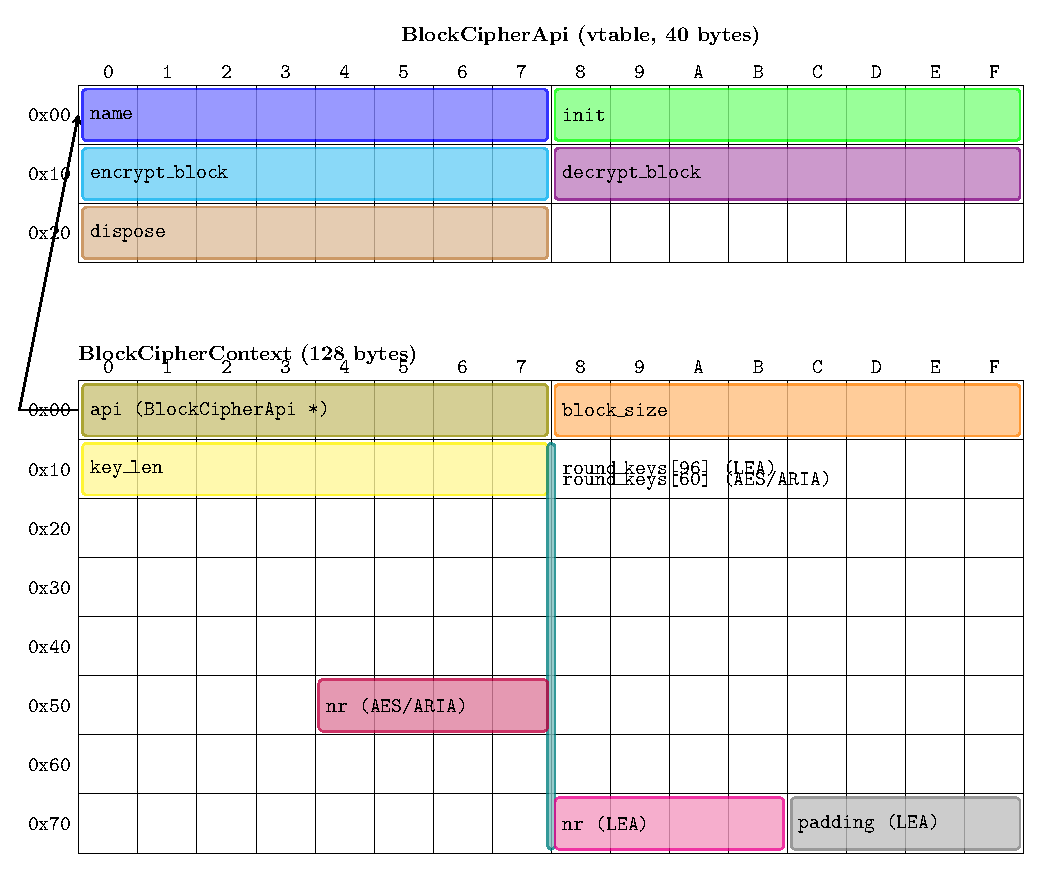
\includegraphics[scale=1]{memory_layout/BlockCipherApi.pdf}
%\end{figure}

\newpage
\begin{lstlisting}[style=cstyle, caption={include/block\_cipher/api\_block\_cipher.h}, captionpos=t]
/* Forward declaration for the context. */
typedef struct __BlockCipherContext__ BlockCipherContext;

typedef struct __BlockCipherApi__ {
	const char *cipher_name; /* e.g. "AES" or "MyCipher" */
	
	block_cipher_status_t (*cipher_init)(
		BlockCipherContext* cipher_ctx, 
		const u8* key, 
		size_t key_len, 
		size_t block_len, 
		BlockCipherDirection dir);
	block_cipher_status_t (*cipher_process)(
		BlockCipherContext* cipher_ctx, 
		const u8* in, 
		u8* out, 
		BlockCipherDirection dir);
	void (*cipher_dispose)(BlockCipherContext* cipher_ctx);
} BlockCipherApi;

typedef union __CipherInternal__ {
	struct __aes_internal__ {
		size_t block_size;      /* Typically must be 16 for AES */
		size_t key_len;         /* 16, 24, or 32 for AES-128/192/256 */
		/* max 60 for AES-256 */
		u32 round_keys[4 * (AES256_NUM_ROUNDS + 1)];     
		int nr;                 /* e.g., 10 for AES-128, 12, or 14... */
	} aes_internal;
	struct __aria_internal__ {
		size_t block_size;      /* Typically must be 16 for ARIA */
		size_t key_len;         /* 16, 24, or 32 for ARIA-128/192/256 */
		/* max 68 for ARIA-256 */
		u32 round_keys[4 * (ARIA256_NUM_ROUNDS + 1)];     
		int nr;                 /* e.g., 12 for ARIA-128, 14, or 16... */
	} aria_internal;
	struct __lea_internal__ {
		size_t block_size;      /* Typically must be 16 for LEA */
		size_t key_len;         /* 16, 24, or 32 for LEA-128/192/256 */
		/* max 192 for LEA-256 */
		u32 round_keys[6 * LEA256_NUM_ROUNDS];    
		int nr;                 /* e.g., 24 for LEA-128, 28, or 32... */
	} lea_internal;
} CipherInternal;

struct __BlockCipherContext__ {
	const BlockCipherApi *cipher_api;  
	CipherInternal cipher_state; /* Generic internal state for any cipher */
};
\end{lstlisting}

\begin{table}[h!]\centering
	\begin{tabular*}{\linewidth}{@{\extracolsep{\fill}}l|p{11cm}||l}
		\toprule
		Subsection & Description & Status \\
		\midrule
		2.1.1     & AES (Advanced Encryption Standard) & Drafted      \\
		2.1.2     & ARIA (Academy, Research Institute, and Agency)  & Drafted \\
		2.1.3     & LEA (Lightweight Encryption Algorithm) & Drafted \\
		\bottomrule
	\end{tabular*}
\end{table}
\newpage
\subsection{AES (Advanced Encryption Standard)}
\begin{table}[h!]
	\centering
	\renewcommand{\arraystretch}{1.25} % Increase row height
	\caption{Parameters of the Block Cipher AES (1-word = 32-bit)}
	\begin{tabular*}{\textwidth}{@{\extracolsep{\fill}}c c c c c c c}
		\toprule[1.2pt]
		\textbf{Alg.} & $\boldsymbol{n}$ (bit) & $\boldsymbol{k}$ (bit) & \textbf{\# of Rounds} & \textbf{RK Size} (bit) & \textbf{\# of RKs} & \textbf{Total RK Size} (bit) \\
		\midrule
		\textsf{AES--128} & 128 & 128 & 10 & 128 (4-word) & 11 & 1408 (44-word) \\
		\textsf{AES--192} & 128 & 192 & 12 & 128 (4-word) & 13 & 1664 (52-word) \\
		\textsf{AES--256} & 128 & 256 & 14 & 128 (4-word) & 15 & 1920 (60-word) \\
		\bottomrule[1.2pt]
	\end{tabular*}
\end{table}

%\begin{table}[h!]\centering\renewcommand{\arraystretch}{1.25} % Increase row height by 1.5 times
%	\caption{Parameters of the Block Cipher AES (1-word = 32-bit)}
%	\begin{tabular*}{\textwidth}{@{\extracolsep{\fill}}c||cccccc}
%		\toprule[1.2pt]
%		\multirow{3}{*}{Algorithms} & Block & Key & Number of & Round-Key & Number of & Total Size of\\
%		& Size & Length & Rounds &  Length & Round-Keys & Round-Keys \\
%		& ($N_b$-word) & ($N_k$-word) & ($N_r$)& (word) & ($N_r+1$)& ($N_b(N_r+1)$)\\
%		\hline\hline
%		\textsf{AES-128} & 4 & 4 & 10 & 4 & 11 & 44 (176-byte) \\
%		\textsf{AES-192} & 4 & 6 & 12 & 4 & 13 & 52 (208-byte) \\
%		\textsf{AES-256} & 4 & 8 & 14 & 4 & 15 & 60 (240-byte) \\
%		\bottomrule[1.2pt]
%	\end{tabular*}
%\end{table}

%\begin{tikzpicture}[>=stealth, node distance=0cm, scale=.9]
%	% Set font for nodes to a small monospace for clarity
%	\tikzstyle{every node}=[font=\footnotesize\ttfamily]
%	
%	% Dimensions and coordinates (assuming 64-bit, pointer = 8 bytes)
%	\def\ptrSize{0.5}    % height for an 8-byte field (in cm)
%	\def\ctxWidth{5.0}   % width of the BlockCipherContext struct box (in cm)
%	\def\apiWidth{4.0}   % width of the BlockCipherApi struct box (in cm)
%	
%	% BlockCipherContext structure box
%	\coordinate (ctxOrigin) at (0,0);                            % top-left corner of BlockCipherContext
%	\draw[draw, thick] (ctxOrigin) rectangle ++(\ctxWidth,-\ptrSize)
%	node[midway] {BlockCipherApi *api};                   % api pointer field
%	\draw[draw, thick] (0,-\ptrSize) rectangle ++(\ctxWidth,-5.0) 
%	node[midway] {uint8\_t internal\_data[256]};             % internal_data array field (256 bytes)
%	\draw[thick] (ctxOrigin) -- ++(0, -5.5);                     % left boundary line for context (extend to full height)
%	\draw[thick] (\ctxWidth, 0) -- ++(0, -5.5);                  % right boundary line for context
%	
%	% Offset markers for BlockCipherContext
%	\draw[thick] ($(ctxOrigin) + (0,0)$) -- ++(-3mm,0) node[left] {0x00};
%	\draw[thick] ($(ctxOrigin) + (0,-\ptrSize)$) -- ++(-3mm,0) node[left] {0x08};
%	\draw[thick] ($(ctxOrigin) + (0,-5.5)$) -- ++(-3mm,0) node[left] {0x108};
%	\draw[decorate, decoration={brace, amplitude=4pt}, thick]
%	(\ctxWidth + 0.1, -\ptrSize) -- node[right=4pt]{256 bytes} (\ctxWidth + 0.1, -5.5);
%	
%	% Label the struct
%	\node[above=2mm of ctxOrigin, anchor=west, font=\normalsize\bfseries] {BlockCipherContext (in memory)};
%	
%	% BlockCipherApi structure box (positioned to the right of context)
%	\coordinate (apiOrigin) at (\ctxWidth + 3.0, 0);            % top-left corner of BlockCipherApi (some gap to the right)
%	% Draw each field of BlockCipherApi as a rectangle
%	\draw[draw, thick] (apiOrigin) rectangle ++(\apiWidth,-\ptrSize)  
%	node[midway] {const char *name};
%	\draw[draw, thick] ($(apiOrigin)+(0,-\ptrSize)$) rectangle ++(\apiWidth,-\ptrSize)  
%	node[midway] {init};
%	\draw[draw, thick] ($(apiOrigin)+(0,-2*\ptrSize)$) rectangle ++(\apiWidth,-\ptrSize)  
%	node[midway] {encrypt\_block};
%	\draw[draw, thick] ($(apiOrigin)+(0,-3*\ptrSize)$) rectangle ++(\apiWidth,-\ptrSize)  
%	node[midway] {decrypt\_block};
%	\draw[draw, thick] ($(apiOrigin)+(0,-4*\ptrSize)$) rectangle ++(\apiWidth,-\ptrSize)  
%	node[midway] {dispose};
%	\draw[thick] (apiOrigin) -- ++(0, -5*\ptrSize);              % left boundary line for API struct
%	\draw[thick] ($(apiOrigin)+(\apiWidth,0)$) -- ++(0, -5*\ptrSize); % right boundary line for API struct
%	
%	% Offset markers for BlockCipherApi
%	\draw[thick] ($(apiOrigin) + (0,0)$) -- ++(-3mm,0) node[left] {0x00};
%	\draw[thick] ($(apiOrigin) + (0,-\ptrSize)$) -- ++(-3mm,0) node[left] {0x08};
%	\draw[thick] ($(apiOrigin) + (0,-2*\ptrSize)$) -- ++(-3mm,0) node[left] {0x10};
%	\draw[thick] ($(apiOrigin) + (0,-3*\ptrSize)$) -- ++(-3mm,0) node[left] {0x18};
%	\draw[thick] ($(apiOrigin) + (0,-4*\ptrSize)$) -- ++(-3mm,0) node[left] {0x20};
%	\draw[thick] ($(apiOrigin) + (0,-5*\ptrSize)$) -- ++(-3mm,0) node[left] {0x28};
%	
%	% Label the struct
%	\node[above=2mm of apiOrigin, anchor=west, font=\normalsize\bfseries] {BlockCipherApi (in memory)};
%	
%	% Pointer arrow from BlockCipherContext.api to BlockCipherApi struct
%	\coordinate (ctxApiPtr) at ($(ctxOrigin) + (\ctxWidth/2, -\ptrSize/2)$);   % center of ctx.api field
%	\coordinate (apiNameLeft) at ($(apiOrigin) + (0, -\ptrSize/2)$);           % left edge midpoint of API.name field
%	\draw[->, thick] (ctxApiPtr) -- (apiNameLeft);
%	
%	% Pointer arrow from BlockCipherApi.name to an example name string
%	\coordinate (apiNameRight) at ($(apiOrigin) + (\apiWidth, -\ptrSize/2)$);
%	\draw[->, thick] (apiNameRight) -- ++(1.5, 0) node[right] {“AES-128”};
%	
%	% Pointer arrows from function pointers to function code (illustrative)
%	\foreach \i/\name in {1/init(), 2/encrypt\_block(), 3/decrypt\_block(), 4/dispose()} {%
%		\coordinate (fieldRight\i) at ($(apiOrigin) + (\apiWidth, -\i*\ptrSize + \ptrSize/2)$);
%		\draw[->, thick] (fieldRight\i) -- ++(1.2, 0) node[right] {\name \,function};
%	}
%	
%	% Legend / notes
%	\node[anchor=west] at ($(ctxOrigin) + (0,-6.2)$) 
%	{\textit{Note: Arrows show pointer targets. “init() function” etc. indicate the actual code for those function pointers.}};
%\end{tikzpicture}
%
%% TikZ diagram of BlockCipherContext and BlockCipherApi (vtable) memory layout
%% (Assuming 64-bit system: pointers are 8 bytes, hence offsets increment by 0x08)
%\begin{tikzpicture}[font=\footnotesize\ttfamily, >=Stealth, scale=.8]
%	% Define dimensions
%	\def\ptrH{0.3}      % height for one pointer field (represents 8 bytes)
%	\def\halfPtrH{0.15} % half of pointer field height
%	\def\intH{9.6}      % height for 256-byte internal_data field (32 * \ptrH)
%	\def\halfIntH{4.8}  % half of internal_data field height
%	\def\ctxWidth{5}    % width of structure boxes
%	\def\vtWidth{5}
%	\def\funcWidth{5.5} % width of function implementation boxes
%	% X-coordinates for structures
%	\def\ctxX{0}        % BlockCipherContext X position
%	\def\vtX{6.5}       % BlockCipherApi (vtable) X position
%	\def\funcX{13}      % Function implementations X position
%	
%	% BlockCipherContext structure outline
%	\draw (\ctxX, 0) rectangle ({\ctxX + \ctxWidth}, {-(\ptrH + \intH)});
%	\draw (\ctxX, -\ptrH) -- ({\ctxX + \ctxWidth}, -\ptrH);  % divider between fields
%	% BlockCipherContext field labels
%	\node[anchor=west, inner sep=1mm] at (\ctxX, -\halfPtrH) {BlockCipherApi *api};
%	\node[anchor=west, inner sep=1mm] at (\ctxX, {-(\ptrH + \halfIntH)}) {u8 internal\_data[256]};
%	% BlockCipherContext offset labels (left side)
%	\node[anchor=east, fill=white, inner sep=1pt] at (\ctxX, 0) {0x00};
%	\node[anchor=east, fill=white, inner sep=1pt] at (\ctxX, -\ptrH) {0x08};
%	\node[anchor=east, fill=white, inner sep=1pt] at (\ctxX, {-(\ptrH + \intH)}) {0x108};
%	% BlockCipherContext size annotations (right side)
%	\node[anchor=west] at ({\ctxX + \ctxWidth + 1mm}, {-\halfPtrH - 0.05}) {8 bytes};
%	\node[anchor=west] at ({\ctxX + \ctxWidth + 1mm}, {-(\ptrH + \halfIntH)}) {256 bytes};
%	
%	% BlockCipherApi (vtable) structure outline
%	\draw (\vtX, 0) rectangle ({\vtX + \vtWidth}, {-5 * \ptrH});
%	\foreach \i in {1,...,4} { % horizontal lines for each vtable field
%		\draw (\vtX, {-\i * \ptrH}) -- ({\vtX + \vtWidth}, {-\i * \ptrH});
%	}
%	% BlockCipherApi vtable field labels
%	\node[anchor=west, inner sep=1mm] at (\vtX, -\halfPtrH) {const char *name};
%	\node[anchor=west, inner sep=1mm] at (\vtX, {-(1 * \ptrH + \halfPtrH)}) {init (function ptr)};
%	\node[anchor=west, inner sep=1mm] at (\vtX, {-(2 * \ptrH + \halfPtrH)}) {encrypt\_block (function ptr)};
%	\node[anchor=west, inner sep=1mm] at (\vtX, {-(3 * \ptrH + \halfPtrH)}) {decrypt\_block (function ptr)};
%	\node[anchor=west, inner sep=1mm] at (\vtX, {-(4 * \ptrH + \halfPtrH)}) {dispose (function ptr)};
%	% BlockCipherApi vtable offset labels (left side)
%	\node[anchor=east, fill=white, inner sep=1pt] at (\vtX, 0) {0x00};
%	\node[anchor=east, fill=white, inner sep=1pt] at (\vtX, { -1 * \ptrH }) {0x08};
%	\node[anchor=east, fill=white, inner sep=1pt] at (\vtX, { -2 * \ptrH }) {0x10};
%	\node[anchor=east, fill=white, inner sep=1pt] at (\vtX, { -3 * \ptrH }) {0x18};
%	\node[anchor=east, fill=white, inner sep=1pt] at (\vtX, { -4 * \ptrH }) {0x20};
%	\node[anchor=east, fill=white, inner sep=1pt] at (\vtX, { -5 * \ptrH }) {0x28};
%	% Brace to label the vtable structure
%	\draw[decorate, decoration={brace, mirror, amplitude=5pt}] (\vtX, { -5 * \ptrH }) -- (\vtX, 0)
%	node[midway, left=6pt]{BlockCipherApi (vtable)};
%	
%	% AES function implementation blocks
%	\node[draw, minimum width=\funcWidth cm, anchor=west, align=left, inner sep=2mm] (funcInit) 
%	at (\funcX, {-(1 * \ptrH + \halfPtrH)}) {aes\_init function implementation};
%	\node[draw, minimum width=\funcWidth cm, anchor=west, align=left, inner sep=2mm] (funcEnc)  
%	at (\funcX, {-(2 * \ptrH + \halfPtrH)}) {aes\_encrypt function implementation};
%	\node[draw, minimum width=\funcWidth cm, anchor=west, align=left, inner sep=2mm] (funcDec)  
%	at (\funcX, {-(3 * \ptrH + \halfPtrH)}) {aes\_decrypt function implementation};
%	\node[draw, minimum width=\funcWidth cm, anchor=west, align=left, inner sep=2mm] (funcDisp) 
%	at (\funcX, {-(4 * \ptrH + \halfPtrH)}) {aes\_dispose function implementation};
%	
%	% Pointer arrows showing relationships
%	\draw[->] ({\ctxX + \ctxWidth}, {-\halfPtrH}) -- (\vtX, {-\halfPtrH});
%	\draw[->] ({\vtX + \vtWidth}, {-(1 * \ptrH + \halfPtrH)}) -- (funcInit.west);
%	\draw[->] ({\vtX + \vtWidth}, {-(2 * \ptrH + \halfPtrH)}) -- (funcEnc.west);
%	\draw[->] ({\vtX + \vtWidth}, {-(3 * \ptrH + \halfPtrH)}) -- (funcDec.west);
%	\draw[->] ({\vtX + \vtWidth}, {-(4 * \ptrH + \halfPtrH)}) -- (funcDisp.west);
%\end{tikzpicture}


\begin{lstlisting}[style=cstyle, caption={include/block\_cipher/block\_cipher\_aes.h}, captionpos=t]
/* Get the AES block cipher vtable. */
const BlockCipherApi* get_aes_api(void);

void aes_set_encrypt_key(const u8 *key, size_t bytes, u32 *rk);
void aes_set_decrypt_key(const u8 *key, size_t bytes, u32 *rk);
void aes_encrypt(const u8 *in, u8 *out, const u32 *rk, int r);
void aes_decrypt(const u8 *in, u8 *out, const u32 *rk, int r);
\end{lstlisting}
\begin{lstlisting}[style=cstyle, caption={src/block\_cipher/block\_cipher\_aes.c}, captionpos=t]
/* Forward declarations of static functions. */
static block_cipher_status_t aes_init(
	BlockCipherContext *ctx, 
	const u8 *key, 
	size_t key_len, 
	size_t block_len, 
	BlockCipherDirection dir);
static block_cipher_status_t aes_process(
	BlockCipherContext *ctx, 
	const u8 *in,
	u8 *out, 
	BlockCipherDirection dir);
static void aes_dispose(BlockCipherContext *ctx);

/* The AES block cipher API. */
static const BlockCipherApi AES_API = {
	.cipher_name          = "AES",
	.cipher_init          = aes_init,
	.cipher_process       = aes_process,
	.cipher_dispose       = aes_dispose
};

/* Get the AES block cipher API. */
const BlockCipherApi *get_aes_api(void) { return &AES_API; }
\end{lstlisting}
\newpage

%\begin{lstlisting}
%/* 
%* AES Round Transformation (Highly Optimized)
%* 
%* I utilized loop unrolling, pointer arithmetic, and 
%* specific compiler extensions to ensure minimal overhead.
%* This is a simplified excerpt focusing on 128-bit keys.
%*/
%
%#include <stdint.h>
%#include <stddef.h>
%
%/* Example S-box for AES; typically a static const table. */
%static const uint8_t sbox[256] = {
%	/* 256 values omitted for brevity ... */
%};
%
%/* 
%* Inline function for SubBytes step using the S-box 
%* Leveraging GCC's __restrict to hint pointer usage.
%*/
%static inline void sub_bytes(uint8_t *__restrict block) {
%	for (int i = 0; i < 16; ++i) {
%		block[i] = sbox[block[i]];
%	}
%}
%
%/*
%* Inlined function for ShiftRows step.
%* Shifts the rows of the 4x4 byte matrix left by
%* varying offsets (0,1,2,3).
%*/
%static inline void shift_rows(uint8_t *__restrict block) {
%	/* Row 1 shift: 4 bytes are rearranged as needed */
%	uint8_t temp = block[1];
%	block[1]     = block[5];
%	block[5]     = block[9];
%	block[9]     = block[13];
%	block[13]    = temp;
%	
%	/* Row 2 shift: 4 bytes swap in pairs */
%	uint8_t temp1 = block[2];
%	uint8_t temp2 = block[6];
%	block[2]      = block[10];
%	block[6]      = block[14];
%	block[10]     = temp1;
%	block[14]     = temp2;
%	
%	/* Row 3 shift: 4 bytes are rearranged again */
%	temp          = block[3];
%	block[3]      = block[15];
%	block[15]     = block[11];
%	block[11]     = block[7];
%	block[7]      = temp;
%}
%
%/* 
%* Multiply operation in GF(2^8) for MixColumns 
%* using a small lookup to accelerate. 
%*/
%static inline uint8_t gm_mul(uint8_t a, uint8_t b) {
%	uint8_t r = 0;
%	for (int i = 0; i < 8; i++) {
%		if (b & 1) r ^= a;
%		uint8_t hi = (uint8_t)(a & 0x80);
%		a <<= 1;
%		if (hi) a ^= 0x1b; 
%		b >>= 1;
%	}
%	return r;
%}
%
%/*
%* MixColumns uses the gf_mul helper for each column in the block.
%* Four 4-byte columns are processed. This routine is unrolled 
%* for maximum performance with minimal overhead.
%*/
%static inline void mix_columns(uint8_t *__restrict block) {
%	for (int col = 0; col < 4; col++) {
%		uint8_t *c = block + (col << 2);
%		uint8_t a0 = c[0], a1 = c[1], a2 = c[2], a3 = c[3];
%		uint8_t r0 = gm_mul(a0, 2) ^ gm_mul(a1, 3) ^ a2 ^ a3;
%		uint8_t r1 = a0 ^ gm_mul(a1, 2) ^ gm_mul(a2, 3) ^ a3;
%		uint8_t r2 = a0 ^ a1 ^ gm_mul(a2, 2) ^ gm_mul(a3, 3);
%		uint8_t r3 = gm_mul(a0, 3) ^ a1 ^ a2 ^ gm_mul(a3, 2);
%		c[0] = r0; c[1] = r1; c[2] = r2; c[3] = r3;
%	}
%}
%
%/*
%* add_round_key merges the round subkey using XOR 
%* for the final step of each round.
%*/
%static inline void add_round_key(uint8_t *block, const uint8_t *round_key) {
%	for (int i = 0; i < 16; ++i) {
%		block[i] ^= round_key[i];
%	}
%}
%
%/*
%* This function performs one AES round:
%* SubBytes -> ShiftRows -> MixColumns -> AddRoundKey
%*/
%void aes_round_optimized(uint8_t *block, const uint8_t *round_key) {
%	sub_bytes(block);
%	shift_rows(block);
%	mix_columns(block);
%	add_round_key(block, round_key);
%}
%\end{lstlisting}

%\paragraph{Discussion of Optimization Techniques}
%
%\begin{itemize}
%	\item \textbf{Loop Unrolling:} By explicitly unrolling small loops (e.g., in \texttt{mix\_columns}), I minimized overhead and allowed the compiler to optimize register usage.
%	\item \textbf{Inline Functions:} Using \texttt{static inline} for repeated sub-steps avoids function-call overhead and permits further inlining by the compiler.
%	\item \textbf{\_\_restrict Keyword:} This GNU C extension hints that pointers do not overlap, helping the compiler optimize more aggressively.
%	\item \textbf{Pointer Arithmetic:} Rather than indexing in 2D, I calculated offsets with \texttt{block + (col << 2)} to reduce overhead and help the compiler precompute certain expressions.
%	\item \textbf{Bitwise Operations:} The gf\_mul routine is carefully written to exploit bit shifts and XOR in a constant-time style, though actual side-channel resistance may need further architecture-specific measures.
%\end{itemize}
%
%Although this code snippet is simplified to illustrate the core round transformation, the real library includes full key scheduling, final rounds (without \texttt{mix\_columns}), and thorough security reviews to avoid side-channel leaks.
%
%\paragraph{Security Considerations}
%
%Since cryptographic code can be sensitive to timing and side-channel attacks, I took these protective measures:
%
%\begin{itemize}
%	\item \textbf{Constant-Time Operations:} The S-box lookups and \texttt{gm\_mul} attempts to avoid data-dependent branching, though further hardware-specific adjustments may be necessary.
%	\item \textbf{Memory Clearing:} I zeroize key data in memory immediately when it is no longer needed, using a dedicated function that the compiler does not optimize away.
%	\item \textbf{Limited Exposure:} The internal routines are compiled as static where possible, preventing accidental usage from outside code.
%\end{itemize}
%
%\paragraph{Test Vectors}
%
%I used known NIST AES test vectors to verify correctness. The makefile includes a \texttt{make test} target that runs a C-based unit test suite, verifying:
%
%\begin{itemize}
%	\item \textbf{AES Single-Block Encryption:} Matches official known-answer tests.
%	\item \textbf{Randomized Stress Tests:} Random keys and plaintexts are encrypted and decrypted to ensure \texttt{plaintext == decryptedCiphertext}.
%\end{itemize}
%
%\paragraph{Performance Testing}
%I relied on microbenchmarking to confirm that the unrolled loops and inline expansions yielded measurable performance gains. For large data sets, using hardware instructions (e.g., AES-NI on x86) could further boost throughput, so the code checks CPU features at runtime if built with hardware-acceleration support.
%
%\paragraph{How I Maintained and Deployed the Module}
%
%From the earliest design stages, I versioned the module in a private Git repository. Whenever I introduced a new optimization or cryptographic transform, I documented it in the commit log, explaining my rationale and the performance or security impact.
%
%Once I gained confidence in the stability of the code, I created release tags (e.g., \texttt{v1.0}, \texttt{v1.1}), each accompanied by a changelog. For deployment within other projects, I have a \texttt{.pc} pkg-config file that allows easy \texttt{pkg-config --cflags --libs crypto\_module} usage, especially on Linux-based environments.
%
%\paragraph{Conclusions and Future Work}
%
%In this manual, I walked through my cryptographic C module from inception to deployment, describing in the first person how I wrote extremely optimized routines and upheld security best practices. Looking forward, I plan to:
%
%\begin{itemize}
%	\item Add alternative ciphers (e.g., ChaCha20) for platforms lacking AES hardware acceleration.
%	\item Improve side-channel countermeasures for hardware traces.
%	\item Integrate a robust test harness with fuzzing to detect memory safety bugs.
%\end{itemize}
%
%I hope that by sharing my insights on performance tuning, memory-safe design, and cryptographic caution, you find this module useful and educational.
%
%%\appendix
%\paragraph{Appendix: Example Build Script}
%
%Below is a small snippet of a \texttt{Makefile} portion I use to build and test the library:
%
%\begin{lstlisting}[language=make]
%CC      := gcc
%CFLAGS  := -O3 -Wall -Wextra -std=c11
%
%LIBNAME := libcrypto_module.a
%
%OBJS := aes_core.o test_vectors.o
%
%all: $(LIBNAME)
%
%$(LIBNAME): $(OBJS)
%@ar rcs $@ $^
%
%test: all
%@$(CC) $(CFLAGS) -o test_crypto test_main.c $(LIBNAME)
%@./test_crypto
%
%clean:
%rm -f $(OBJS) $(LIBNAME) test_crypto
%\end{lstlisting}
%
%\textbf{Usage}:
%\begin{verbatim}
%$ make
%$ make test
%\end{verbatim}
%
%\paragraph{References}
%
%\begin{itemize}
%	\item \textbf{NIST AES Standard:} \href{https://nvlpubs.nist.gov/nistpubs/FIPS/NIST.FIPS.197.pdf}{FIPS-197 (AES)}
%	\item \textbf{Intel AES-NI Reference:} \href{https://www.intel.com/content/www/us/en/developer/articles/technical/intel-advanced-encryption-standard-aes-instructions-set.html}{Intel AES-NI Docs}
%	\item \textbf{GNU Compiler Docs:} \href{https://gcc.gnu.org/onlinedocs/}{\texttt{gcc} Online Documentation}
%\end{itemize}

\subsection{ARIA (Academy, Research Institute, and Agency)}
\begin{table}[h!]
	\centering
	\renewcommand{\arraystretch}{1.25} % Increase row height
	\caption{Parameters of the Block Cipher ARIA (1-word = 32-bit)}
	\begin{tabular*}{\textwidth}{@{\extracolsep{\fill}}c c c c c c c}
		\toprule[1.2pt]
		\textbf{Alg.} & $\boldsymbol{n}$ (bit) & $\boldsymbol{k}$ (bit) & \textbf{\# of Rounds} & \textbf{RK Size} (bit) & \textbf{\# of RKs} & \textbf{Total RK Size} (bit) \\
		\midrule
		\textsf{ARIA--128} & 128 & 128 & 12 & 128 (4-word) & 13 & 1664 (52-word) \\
		\textsf{ARIA--192} & 128 & 192 & 14 & 128 (4-word) & 15 & 1920 (60-word) \\
		\textsf{ARIA--256} & 128 & 256 & 16 & 128 (4-word) & 17 & 2176 (68-word) \\
		\bottomrule[1.2pt]
	\end{tabular*}
\end{table}
\begin{lstlisting}[style=cstyle, caption={include/block\_cipher/block\_cipher\_aria.h}, captionpos=t]
/* Get the ARIA block cipher vtable. */
const BlockCipherApi* get_aria_api(void);

void aria_set_encrypt_key(const u8 *key, size_t bytes, u32 *rk);
void aria_set_decrypt_key(const u8 *key, size_t bytes, u32 *rk);
void aria_encrypt(const u8 *in, u8 *out, const u32 *rk, int r);
void aria_decrypt(const u8 *in, u8 *out, const u32 *rk, int r);
\end{lstlisting}
\begin{lstlisting}[style=cstyle, caption={src/block\_cipher/block\_cipher\_aria.c}, captionpos=t]
/* Forward declarations of static functions. */
static block_cipher_status_t aria_init(
	BlockCipherContext *ctx, 
	const u8 *key, 
	size_t key_len, 
	size_t block_len, 
BlockCipherDirection dir);
static block_cipher_status_t aria_process(
	BlockCipherContext *ctx, 
	const u8 *in, 
	u8 *out, 
	BlockCipherDirection dir);
static void aria_dispose(BlockCipherContext *ctx);

/* The ARIA block cipher API. */
static const BlockCipherApi ARIA_API = {
	.cipher_name    = "ARIA",
	.cipher_init    = aria_init,
	.cipher_process = aria_process,
	.cipher_dispose = aria_dispose
};
/* Get the ARIA block cipher API. */
const BlockCipherApi* get_aria_api(void) { return &ARIA_API; }
\end{lstlisting}

\newpage
\subsection{LEA (Lightweight Encryption Algorithm)}
\begin{table}[h!]
	\centering
	\renewcommand{\arraystretch}{1.25} % Increase row height
	\caption{Parameters of the Block Cipher LEA (1-word = 32-bit)}
	\begin{tabular*}{\textwidth}{@{\extracolsep{\fill}}c c c c c c c}
		\toprule[1.2pt]
		\textbf{Alg.} & $\boldsymbol{n}$ (bit) & $\boldsymbol{k}$ (bit) & \textbf{\# of Rounds} & \textbf{RK Size} (bit) & \textbf{\# of RKs} & \textbf{Total RK Size} (bit) \\
		\midrule
		\textsf{LEA--128}  & 128 & 128 & 24 & 192 (6-word) & 24 & 4608 (144-word) \\
		\textsf{LEA--192}  & 128 & 192 & 28 & 192 (6-word) & 28 & 5376 (168-word) \\
		\textsf{LEA--256}  & 128 & 256 & 32 & 192 (6-word) & 32 & 6144 (192-word) \\
		\bottomrule[1.2pt]
	\end{tabular*}
\end{table}
\begin{lstlisting}[style=cstyle, caption={include/block\_cipher/block\_cipher\_aria.h}, captionpos=t]
/* Get the LEA block cipher vtable. */
const BlockCipherApi* get_lea_api(void);

void lea_set_encrypt_key(const u8 *key, size_t bytes, u32 *rk);
void lea_set_decrypt_key(const u8 *key, size_t bytes, u32 *rk);
void lea_encrypt(const u8 *in, u8 *out, const u32 *rk, int r);
void lea_decrypt(const u8 *in, u8 *out, const u32 *rk, int r);
\end{lstlisting}
\begin{lstlisting}[style=cstyle, caption={src/block\_cipher/block\_cipher\_aria.c}, captionpos=t]
/* Forward declarations of static functions. */
static block_cipher_status_t lea_init(
	BlockCipherContext *ctx, 
	const u8 *key, 
	size_t key_len, 
	size_t block_len, 
	BlockCipherDirection dir);
static block_cipher_status_t lea_process(
	BlockCipherContext *ctx, 
	const u8 *in, 
	u8 *out, 
	BlockCipherDirection dir);
static void lea_dispose(BlockCipherContext *ctx);

/* The LEA block cipher API. */
static const BlockCipherApi LEA_API = {
	.cipher_name          = "LEA",
	.cipher_init          = lea_init,
	.cipher_process       = lea_process,
	.cipher_dispose       = lea_dispose
};
/* Get the LEA block cipher API. */
const BlockCipherApi *get_lea_api(void) { return &LEA_API; }
\end{lstlisting}
% Detailed content about supported block ciphers, usage examples, ASM optimizations

\newpage
%-----------------------------------------------------------------------
%  SECTION 2: MODES OF OPERATION
%-----------------------------------------------------------------------
\section{Modes of Operation}

\begin{lstlisting}[style=cstyle]
typedef struct __ModeOfOperationApi__ {
	const char *name;
	void (*init)( /* ... */ );
	void (*process)( /* ... */ );
	void (*dispose)( /* ... */ );
} ModeOfOperationApi;

typedef union __ModeInternal__ {
	struct __cbc_internal__ {
		/* ... */
	} cbc_internal;
	struct __ctr_internal__ {
		/* ... */
	} ctr_internal;
	struct __gcm_internal__ {
		/* ... */
	} gcm_internal;
	struct __ecb_internal__ {
		/* ... */
	} ecb_internal;
	
} ModeInternal;

typedef struct __ModeOfOperationContext__ {
	const ModeOfOperationApi *api;  // Pointer to the mode API
	BlockCipherContext cipher_ctx; // Block cipher context
	ModeInternal internal_data;     // Internal state for the mode
} ModeOfOperationContext;
\end{lstlisting}
%\begin{figure}[h!]
%	\begin{tikzpicture}[x=1cm, y=-0.07cm, font=\scriptsize, draw=black, >=Stealth, scale=.8]
	% BlockCipherContext outline
	\draw[thick] (0,0) rectangle ++(4,128);  % 128 bytes tall, 3 cm wide
	\draw[thick] (0,8) -- ++(4,0);          % line separating api vs internal_data at 8 bytes
	
	% BlockCipherContext labels and offsets
	\node[anchor=south, align=center, font=\small] at (2,0) {\textbf{ModeOfOperationContext}\\ \textbf{(800=8+792 bytes)}};
	\node[align=center] at (2,4) {\texttt{ModeOfOperationApi*}};
	\node[align=center] at (2,68) {\texttt{CipherInternal}\\ (union, 792 bytes)};
	
	\node[anchor=east] at (0,0) {{\tiny\ttfamily 0x000}};   % top address
	\node[anchor=east] at (0,8) {{\tiny\ttfamily 0x008}};
	\node[anchor=east] at (0,16) {{\tiny\ttfamily 0x010}};
	\node[anchor=east] at (0,24) {{\tiny\ttfamily 0x018}};
	\node[anchor=east] at (0,120) {{\tiny\ttfamily 0x318}};
	\node[anchor=east] at (0,128) {{\tiny\ttfamily 0x320}};
	
	% Expand union internal_data: AES, ARIA, LEA internal structures side-by-side
	% Base alignment line for union (offset 0x08 in context)
	\draw[densely dashed, color=gray!50] (4,8) -- ++(14,0) node[anchor=west]{\tiny\ttfamily 0x008};
	\draw[densely dashed, color=gray!50] (4,16) -- ++(14,0) node[anchor=west]{\tiny\ttfamily 0x010};
	\draw[densely dashed, color=gray!50] (4,24) -- ++(14,0) node[anchor=west]{\tiny\ttfamily 0x018};
	\draw[densely dashed, color=gray!50] (4,45) -- ++(14,0) node[anchor=west]{\tiny\ttfamily 0x108};
	\draw[densely dashed, color=gray!50] (4,53) -- ++(14,0) node[anchor=west]{\tiny\ttfamily 0x110};
	\draw[densely dashed, color=gray!50] (4,75) -- ++(14,0) node[anchor=west]{\tiny\ttfamily 0x128};
	\draw[densely dashed, color=gray!50] (4,83) -- ++(14,0) node[anchor=west]{\tiny\ttfamily 0x130};
	\draw[densely dashed, color=gray!50] (4,120) -- ++(14,0) node[anchor=west]{\tiny\ttfamily 0x318};
	\draw[densely dashed, color=gray!50] (4,128) -- ++(14,0) node[anchor=west]{\tiny\ttfamily 0x320};
	
	% AES internal struct (80 bytes used out of 120)
	\draw (5,8) rectangle ++(3,120);       % union size tall (for visual alignment)
	\draw (5,16) -- ++(3,0);
	\draw (5,24) -- ++(3,0);
	\draw (5,45) -- ++(3,0);
	\draw (5,53) -- ++(3,0);
	\node[anchor=south, align=center] at (6.5,8) {\textbf{aes\_internal}\\ \textbf{(8+8+240+8=264 bytes)}};
	\node at (6.5,12) {\texttt{size\_t block\_size}};
	\node at (6.5,20) {\texttt{size\_t key\_len}};
	\node[align=center] at (6.5,36) {\texttt{u32 round\_keys[60]} \\ (240 bytes)};
	\node at (6.5,49) {\texttt{int nr}\; (4 bytes)};
	\node[color=gray, align=center] at (6.5,90) {\footnotesize (unused\\ \footnotesize 528 bytes)};
	\filldraw[gray!70, opacity=.2] (5, 53) rectangle (8, 128);
	
	\filldraw[teal!70, opacity=.2] (5, 8) rectangle (8, 16);
	\filldraw[orange!70, opacity=.2] (5, 16) rectangle (8, 24);
	\filldraw[red!70, opacity=.2] (5, 24) rectangle (8, 45);
	\filldraw[blue!70, opacity=.2] (5, 45) rectangle (8, 53);
	
	% ARIA internal struct (same as AES, 80 bytes)
	\draw (9,8) rectangle ++(3,120);
	\draw (9,16) -- ++(3,0);
	\draw (9,24) -- ++(3,0);
	\draw (9,75) -- ++(3,0);
	\draw (9,83) -- ++(3,0);
	\node[anchor=south, align=center] at (10.5,8) {\textbf{aria\_internal}\\ \textbf{(8+8+272+8=296 bytes)}};
	\node at (10.5,12) {\texttt{size\_t block\_size}};
	\node at (10.5,20) {\texttt{size\_t key\_len}};
	\node[align=center] at (10.5,50) {\texttt{u32 round\_keys[68]} \\ (272 bytes)};
	\node at (10.5,79) {\texttt{int nr}\; (4 bytes)};
	\node[color=gray, align=center] at (10.5,104) {\footnotesize (unused\\ \footnotesize 496 bytes)};
	\filldraw[gray!70, opacity=.2] (9, 83) rectangle (12, 128);
	
	\filldraw[teal!70, opacity=.2] (9, 8) rectangle (12, 16);
	\filldraw[orange!70, opacity=.2] (9, 16) rectangle (12, 24);
	\filldraw[red!70, opacity=.2] (9, 24) rectangle (12, 75);
	\filldraw[blue!70, opacity=.2] (9, 75) rectangle (12, 83);
	
	% LEA internal struct (116 bytes + 4 bytes padding)
	\draw (13,8) rectangle ++(3,120);
	\draw (13,16) -- ++(3,0);
	\draw (13,24) -- ++(3,0);
	\draw (13,120) -- ++(3,0);
	\node[anchor=south, align=center] at (14.5,8) {\textbf{lea\_internal}\\ \textbf{(8+8+768+8=792 bytes)}};
	\node at (14.5,12) {\texttt{size\_t block\_size}};
	\node at (14.5,20) {\texttt{size\_t key\_len}};
	\node[align=center] at (14.5,64) {\texttt{u32 round\_keys[192]} \\ (768 bytes)};
	\node at (14.5,124) {\texttt{int nr}\; (4 bytes)};
	
	\filldraw[teal!70, opacity=.2] (13, 8) rectangle (16, 16);
	\filldraw[orange!70, opacity=.2] (13, 16) rectangle (16, 24);
	\filldraw[red!70, opacity=.2] (13, 24) rectangle (16, 120);
	\filldraw[blue!70, opacity=.2] (13, 120) rectangle (16, 128);
	
	% Brace to indicate union grouping
	\draw[decorate,decoration={brace,amplitude=4pt}] (16,130) -- node[below=4pt]{Union members (share same memory)} (5,130);
	
	% BlockCipherApi vtable structure (40 bytes)
	% Place vtable below (starting at y=140 for offset 0)
	\filldraw[blue!50, opacity=.8] (0, 160) rectangle (3, 168);
	\draw[thick] (0,160) rectangle ++(3,32);
	\draw[thick] (0,168) -- ++(3,0);
	\draw[thick] (0,176) -- ++(3,0);
	\draw[thick] (0,184) -- ++(3,0);
	%	\draw[thick] (0,192) -- ++(3,0);
	\node[anchor=south,align=center] at (1.5,160) {\textbf{BlockCipherApi (vtable)}\\ \textbf{8$\times$4=32 bytes}};
	\node at (1.5,164) {\texttt{const char* name}};
	\node at (1.5,172) {\texttt{void*}};
	\node at (1.5,180) {\texttt{void*}};
	%	\node at (1.5,188) {\texttt{void*}};
	\node at (1.5,188) {\texttt{void*}};
	
	% Arrows: BlockCipherContext.api -> vtable, and vtable function ptrs -> functions
	% API pointer arrow (from BCC.api field to vtable)
	\draw[->, thick] (0,4) -| (-1,4) -- (-1,164) -- ++(1,0);
	
	% Function implementation nodes for AES
	\node[draw, anchor=west, fill=magenta!10] (fn_init)        at (5,172) {\texttt{aes\_init(BlockCipherContext* ctx, /* ... */ );}};
	\node[draw, anchor=west, fill=green!10] (fn_encrypt)     at (5,180) {\texttt{aes\_process\_block(BlockCipherContext* ctx, /* ... */ );}};
	%	\node[draw, anchor=west, fill=lime!10] (fn_decrypt)     at (3.5,188) {\texttt{decrypt(BlockCipherContext* ctx, const u8* ct, u8* pt);}};
	\node[draw, anchor=west, fill=cyan!10] (fn_dispose)     at (5,188) {\texttt{dispose(BlockCipherContext* ctx);}};
	
	\draw[->] (3,172) -- (fn_init.west);
	\draw[->] (3,180) -- (fn_encrypt.west);
	%	\draw[->] (3,188) -- (fn_decrypt.west);
	\draw[->] (3,188) -- (fn_dispose.west);
\end{tikzpicture}
%\end{figure}

\subsection{Electronic Codebook (ECB)}
TBA
\subsection{Cipher Block Chaining (CBC)}
TBA
\subsection{Counter (CTR)}
TBA
\newpage
\section{Galois\;/\;Counter Mode (GCM)}
%\begin{center}
%	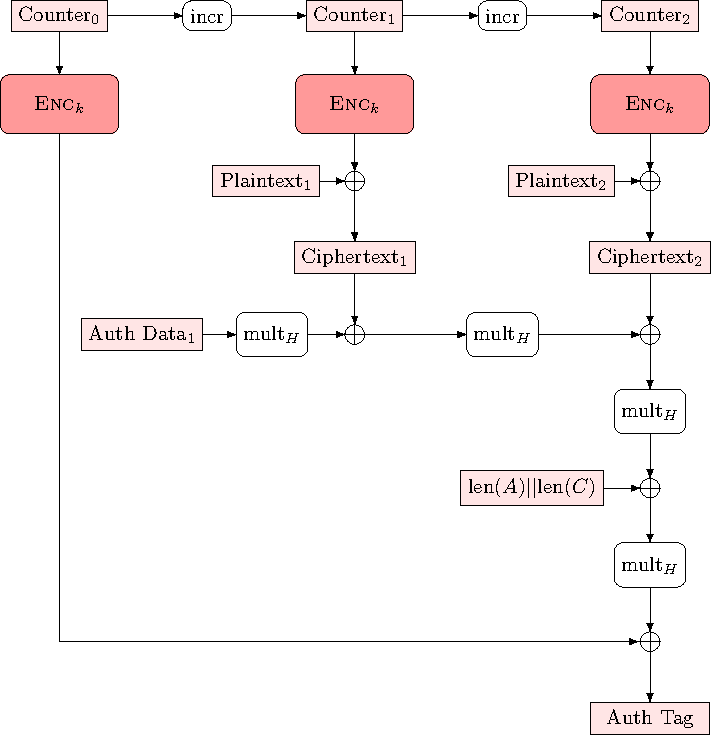
\includegraphics[scale=1]{tikz/GCM_encryption}
%\end{center}

\begin{figure}[h!]\centering
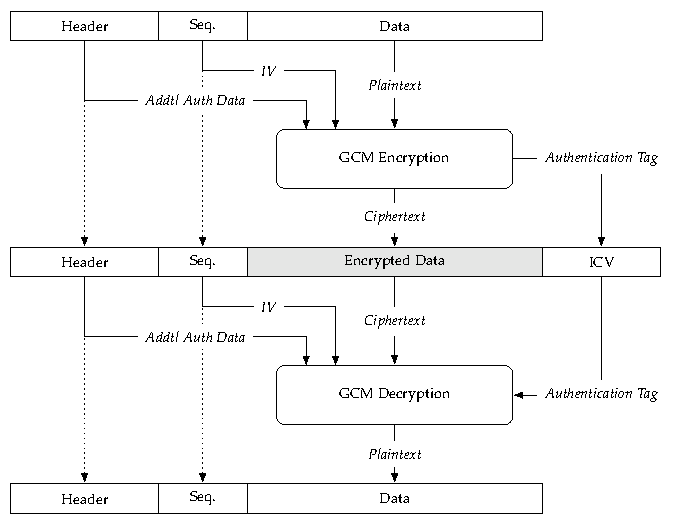
\includegraphics[scale=1.25]{tikz/gcm_mode}
\end{figure}

\subsection{Multiplication in $\GF(2^{128})$}
\begin{definition}
	Let \(\mathbb F_2 = \{0,1\}\) be the field with two elements.  Fix an irreducible polynomial
	\[
	f(x) \;=\; x^{128} + x^7 + x^2 + x + 1 
	\quad\in\; \mathbb F_2[x].
	\]
	Then
	\[
	\mathrm{GF}(2^{128}) \;=\; \mathbb F_2[x] \,\big/\,\bigl(f(x)\bigr)
	\]
	is the degree-\(128\) extension field.
\end{definition}
\begin{remark}
Every element \(\alpha\in\mathrm{GF}(2^{128})\) can be written uniquely as \[
\alpha \;=\; a_{127}x^{127} + a_{126}x^{126} + \cdots + a_1 x + a_0
\quad(a_i\in\{0,1\}).
\] We identify \(\alpha\) with the \(128\)-bit vector \((a_{0},\dots,a_{127})\in\F_2\).
\end{remark}

\paragraph{Polynomial Representation and Reduction}
Multiplication in \(\mathbb F_2[x]\) is carry-less:
\[
\left(\sum_i a_i x^i\right)\cdot\left(\sum_j b_j x^j\right)
=\sum_{i,j}\left(a_i b_j\right)\,x^{i+j}\,,
\]
with all additions mod 2.  To get the product in \(\mathrm{GF}(2^{128})\), we then reduce
the degree-\(\le 254\) result modulo \(f(x)\).

\paragraph{Bit-Level Algorithm}
We implement multiplication by a simple “shift-and-add” method with reduction on each
shift, often called \(\mathtt{xtime}\).

\begin{definition}[\,\(\mathtt{xtime}\) map\,]
	For \(v\in\mathrm{GF}(2^{128})\) represented as a 128-bit word, define
	\[
	\mathtt{xtime}(v) = 
	\begin{cases}
		v \ll 1, &\text{if the MSB of }v\text{ is }0,\\[6pt]
		(v \ll 1)\oplus R, &\text{if the MSB of }v\text{ is }1,
	\end{cases}
	\]
	where \(R\) is the bit-vector corresponding to the reduction polynomial
	\(x^7+x^2+x+1\).
\end{definition}

\paragraph{Pseudocode}
\ \\ \begin{algorithm}[H]
	\caption{Multiply two field elements \(a,b\in\mathrm{GF}(2^{128})\)}
	\label{alg:mul2}
	\begin{algorithmic}[1]
		\REQUIRE \(a,b\in\{0,1\}^{128}\) as 128-bit words  
		\ENSURE \(c = a\cdot b \bmod f(x)\)
		\STATE \(c \leftarrow 0\)  
		\STATE \(v \leftarrow a\)  
		\FOR{\(i=0\) to \(127\)}  
		\IF{bit \(i\) of \(b\) is 1}  
		\STATE \(c \leftarrow c \oplus v\)  
		\ENDIF  
		\STATE \(v \leftarrow \mathtt{xtime}(v)\)  
		\ENDFOR  
		\RETURN \(c\)
	\end{algorithmic}
\end{algorithm}



\paragraph{References:} 
\cite{NIST80038d},\;
\cite{McGrewViega2004gcm}

\newpage
%-----------------------------------------------------------------------
%  CHAPTER 4: RANDOM NUMBER GENERATOR (Placeholder)
%-----------------------------------------------------------------------
\section{Random Number Generator}
TBA
% Implementation details, entropy sources, usage examples

%-----------------------------------------------------------------------
%  CHAPTER 5: HASH FUNCTIONS (Placeholder)
%-----------------------------------------------------------------------
\section{Hash Functions}
\subsection{SHA-2 Algorithms}
TBA
\subsection{SHA-3 Algorithms}
TBA
\subsection{Lightweight Secure Hash (LSH)}
TBA
% Implementation details, supported hashes, ASM notes

%-----------------------------------------------------------------------
%  CHAPTER 6: MESSAGE AUTHENTICATION CODES (Placeholder)
%-----------------------------------------------------------------------
\section{Message Authentication Codes}
TBA
% Content about HMAC, CMAC, usage examples, best practices

%-----------------------------------------------------------------------
%  CHAPTER 7: KEY DERIVATION FUNCTIONS (Placeholder)
%-----------------------------------------------------------------------
\section{Key Derivation Functions}
TBA
% PBKDF, HKDF, usage in password hashing or key expansions

%-----------------------------------------------------------------------
%  CHAPTER 8: KEY EXCHANGE (Placeholder)
%-----------------------------------------------------------------------
\section{Diffie-Hellman Key Exchange}
TBA
% ECDH, DH, usage details, integration

%-----------------------------------------------------------------------
%  CHAPTER 9: SIGNATURE ALGORITHMS (Placeholder)
%-----------------------------------------------------------------------
\section{Signature Algorithms}
TBA
% ECDSA, RSA, usage patterns, performance tips

%%-----------------------------------------------------------------------
%%  CHAPTER 3: BUILD AND INTEGRATION (Placeholder)
%%-----------------------------------------------------------------------
\chapter{Build and Integration}

\section{Makefile Configuration and Overview}
This section describes the build system for the CryptoModule demo, driven by a single GNU Makefile. It covers compiler settings, directory layout, source discovery, and all available targets.

\subsection{Compiler, Flags, and Directories}
\begin{lstlisting}[numbers=none]
# Compiler and flags
CC      := gcc
CFLAGS  := -std=c99 -g -O2 -Wall -Wextra -I. -Iinclude -Isrc

# Executable name
TARGET  := cryptomodule-demo

# Output directories
OBJ_DIR := build
BIN_DIR := bin
\end{lstlisting}
\begin{itemize}
	\item \texttt{gcc} in C99 mode, with debug symbols (\texttt{-g}) and optimization (\texttt{-O2}).
	\item Warnings enabled (\texttt{-Wall -Wextra}), include paths set for project headers.
	\item Object files placed under \texttt{build/}, preserving the \texttt{src/} subdirectory structure; final binary in \texttt{bin/}.
\end{itemize}

\subsection{Automatic Source and Object Discovery}
\begin{lstlisting}[numbers=none]
# Find all .c files in src/ recursively
SRCS := $(shell find src -name '*.c')

# Map src/foo.c -> build/foo.o
OBJS := $(patsubst src/%.c,$(OBJ_DIR)/%.o,$(SRCS))
\end{lstlisting}

\newpage
\subsection{Usage Examples}
\begin{lstlisting}[numbers=none]
###############################################################################
# 1) build : compile + link
###############################################################################
build: $(BIN_DIR)/$(TARGET)

# Link step: gather all objects into a single executable
$(BIN_DIR)/$(TARGET): $(OBJS)
	@echo "[LINK] Linking objects to create $@"
	@mkdir -p $(BIN_DIR)
	$(CC) $(CFLAGS) $^ -o $@
# Compile step: For each .c -> .o
$(OBJ_DIR)/%.o: src/%.c
	@echo "[CC] Compiling $< into $@"
	@mkdir -p $(dir $@)
	$(CC) $(CFLAGS) -c $< -o $@
###############################################################################
# 2) run : run the resulting binary
###############################################################################
run: build
	@echo "[RUN] Running $(BIN_DIR)/$(TARGET)"
	@./$(BIN_DIR)/$(TARGET)

###############################################################################
# 3) clean : remove build artifacts
###############################################################################
clean:
@echo "[CLEAN] Removing build artifacts..."
	rm -rf $(OBJ_DIR) $(BIN_DIR)
	@echo "[CLEAN] Removing *.req and *.rsp files in testvectors folder..."
	find testvectors -type f \( -name '*.req' -o -name '*.rsp' \) -delete

###############################################################################
# 4) rebuild : clean + build
###############################################################################
rebuild: clean build

###############################################################################
# 5) valgrind : run the binary under Valgrind for memory checking
###############################################################################
valgrind: build
	@echo "[VALGRIND] Running Valgrind..."
	valgrind --leak-check=full ./$(BIN_DIR)/$(TARGET)
\end{lstlisting}

\begin{description}
	\item[\texttt{make build}] Compile (\texttt{.c → .o}) and link (\texttt{.o → executable}).
	\item[\texttt{make run}] Build if necessary, then execute \texttt{bin/cryptomodule-demo}.
	\item[\texttt{make clean}] Remove \texttt{build/}, \texttt{bin/}, and any \texttt{*.req}/\texttt{*.rsp} in \texttt{testvectors/}.
	\item[\texttt{make rebuild}] Alias for \texttt{clean} followed by \texttt{build}.
	\item[\texttt{make valgrind}] Build, then run under Valgrind for memory-leak checks.
\end{description}
% Makefile overview, linking instructions, library creation
%
%%-----------------------------------------------------------------------
%%  CHAPTER 4: TESTING (Placeholder)
%%-----------------------------------------------------------------------
%\chapter{Testing}
%% Unit tests, integration tests, reference vectors

%%-----------------------------------------------------------------------
%%  CHAPTER 5: FAQ / TROUBLESHOOTING (Placeholder)
%%-----------------------------------------------------------------------
%\chapter{FAQ / Troubleshooting}
%% Common errors, solutions, performance tuning

\newpage
\section{Example: Main Function for Block‐Cipher KATs}
\begin{lstlisting}[caption={Invoke known-answer tests for AES block ciphers},label={lst:main-kat},captionpos=t]
int main(void) {
	KAT_TEST_BLOCKCIPHER(BLOCK_CIPHER_AES128);
	KAT_TEST_BLOCKCIPHER(BLOCK_CIPHER_AES192);
	KAT_TEST_BLOCKCIPHER(BLOCK_CIPHER_AES256);
	return 0;
}
\end{lstlisting}
\begin{lstlisting}[]
@>$ make rebuild
@>$ make run
\end{lstlisting}

\begin{figure}[h!]\centering
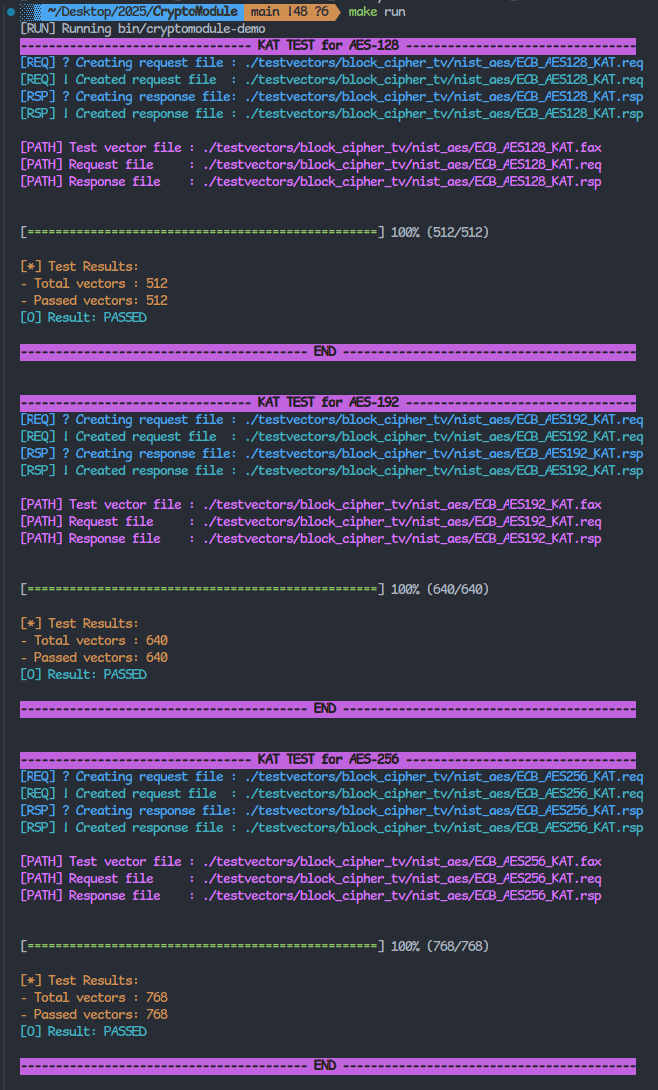
\includegraphics[scale=.65]{images/make_run}
\end{figure}

\newpage
\bibliography{bibliography}

\newpage
\appendix
%-----------------------------------------------------------------------
%  CHAPTER 13: APPENDICES (Placeholder)
%-----------------------------------------------------------------------
\chapter*{Appendices}
TBA
% Glossary, references, external documentation
\end{document}
